\documentclass[main.tex]{subfiles}

\begin{document}
\section{Preliminary Test and Motivation}
The first part of this work was to examine the stability of the reconstructed Crab spectrum looking at the photon index and the integral flux above a threshold value based on the lowest energy where photons were reconstructed across zenith angles. The data used were from nights of horizon-to-horizon Crab runs (Jan 12 2018, Jan 13 2018, and Jan 04, 2019), where Crab runs were taken from the horizon to culmination and back to the horizon.

For Method0, the reconstructed energy spectra appear to be largely stable under variations in zenith angle (Fig. \ref{fig:index_compare} and \ref{fig:intf_compare}). The slopes of the best fit gradient lines are insignificant for both the integral flux above the threshold energy ($10^{0.35} \approx 2.24$TeV) and the spectral index -- as they should be since physically these quantities are independent of zenith angle.

The \disp method is able to reconstruct events down to larger zenith angles than the standard method although lower statistics at large zenith angles lead to larger uncertainties. However, the integral flux from the \disp method fit has a significant positive correlation with zenith angle, and lies significantly below the integral flux reconstructed from Method0.

\begin{figure}[H]
  \begin{center}
    \subfigure[Crab reconstructed spectral index using Method0 and Method5t.]{ 
      \includegraphics[width=0.9\linewidth]{images/Crab_C2C/Index_compare}
      \label{fig:index_compare}
    }  
    \subfigure[Crab reconstructed integral flux above 2.24 TeV ($10^{0.35}$ TeV) using Method0 and Method5t.]{ 
      \includegraphics[width=0.9\linewidth]{images/Crab_C2C/Intf_compare}
      \label{fig:intf_compare}
    }
  \end{center}
  \caption[Crab spectrum reconstruction.]{Reconstruction of the Crab spectrum using Method0 (standard reconstruction from \vegas) and Method5t (\disp).}
  \label{fig:spectrum_compare}
\end{figure}

\section{\disp Table and \rse Dependencies}
This effect in integral flux hints at some systematic effects that are not yet understood. In order to determine and/or resolve the underlying causes, the scripts to generate the BDT weight tables were re-written and the tables generated independently. For the purposes of this work, the 68\% containment radius in angular offset (\rse\hspace{-4pt}) is used as a measure of angular resolution and performance of the reconstruction.

\subsection{Zenith Angle Dependence}
A set of \disp tables was generated with a small sample of events ($n\approx 1.9\e6$) across the range of zenith angles of interest ($20^\circ-65^\circ$). This was compared to the regular \disp method. Since there was no record of the training sample size for the standard tables, this test sample was useful in determining the resolution of the \disp method with a relatively small computational footprint. Additionally, it allowed for some simple tests of dependence of the \disp table on parameters not explicitly in the \disp tables.

The test \disp table and the standard \disp tables were used to reconstruct simulation events and compared with Method0 (the standard method of direction reconstruction). In both cases, the \disp method performs better than Method0 at the largest zenith angles ($\geq 55^\circ$, see \ref{fig:olddisp_ratio}-\ref{fig:disp_ratio_250} for \rse of the \disp methods divided by that for Method0 at the same zenith angle), but the test \disp table fared 30-50\% worse across zenith angles, and for zenith angles in the range $45^\circ-50^\circ$, Method0 performed better than the test model. 

\begin{figure}[htbp]
  \begin{center}
      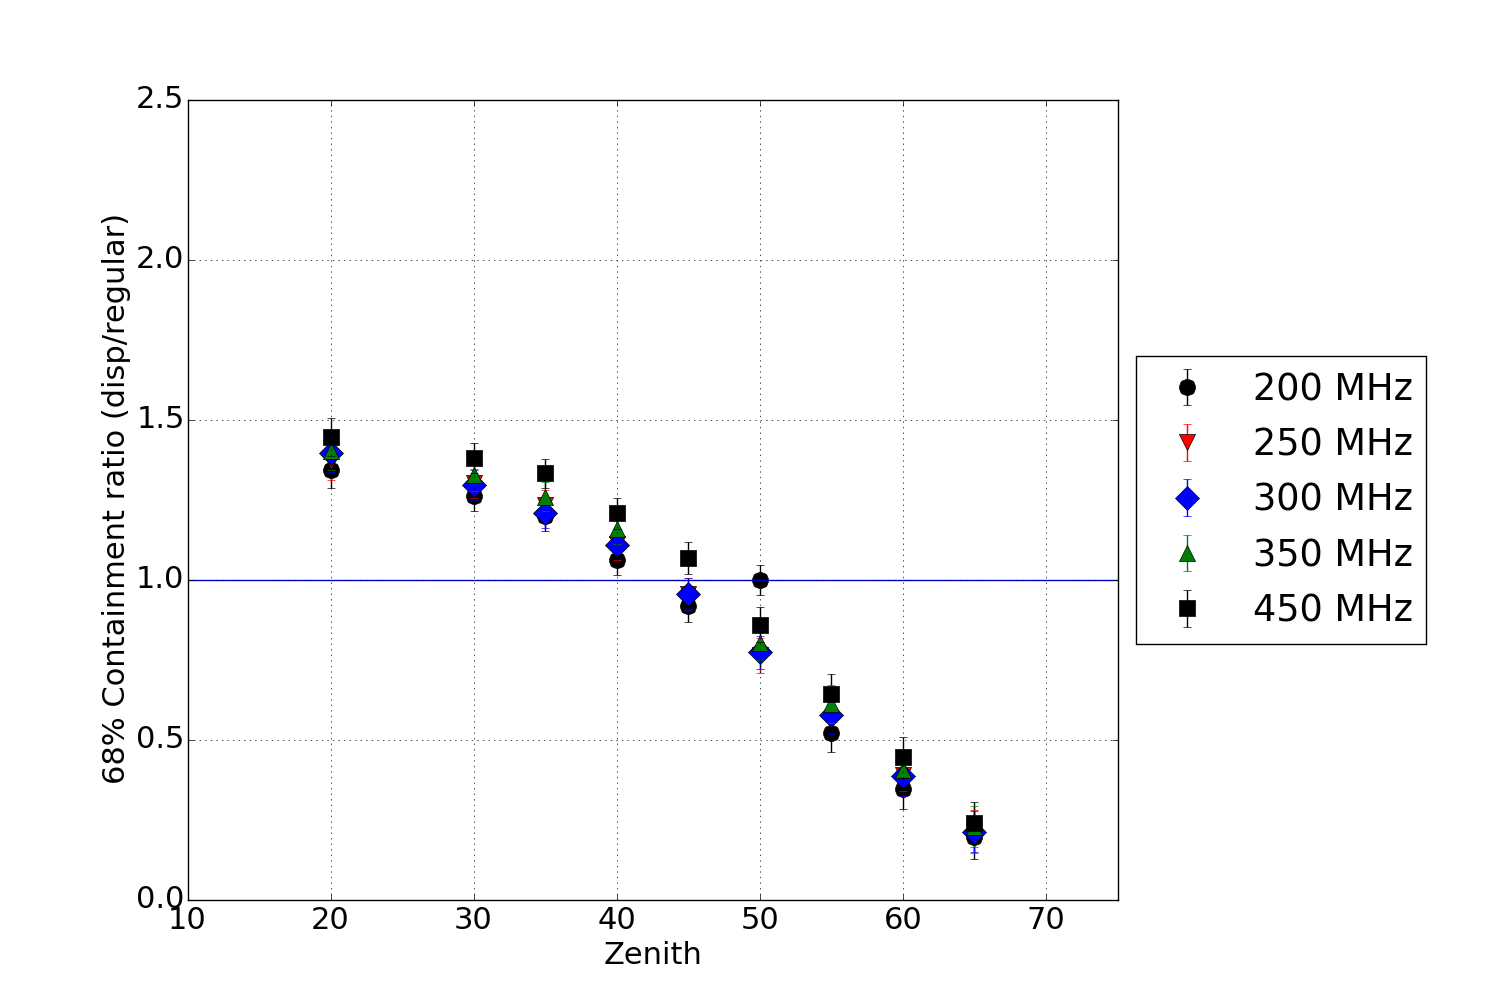
\includegraphics[width=0.8\linewidth]{images/disp_standard_ratio_xzen}
      \caption[``standard'' \disp table reconstruction.]{Ratio of \rse of the ``standard'' \disp table to that from Method0. Since this is the ratio of methods, the horizontal blue line denotes the performance using Method0, and this method performs better than Method0 for zenith $>45^\circ$.}  
      \label{fig:olddisp_ratio}
  \end{center}
\end{figure}

\begin{figure}[htbp]
  \centering
  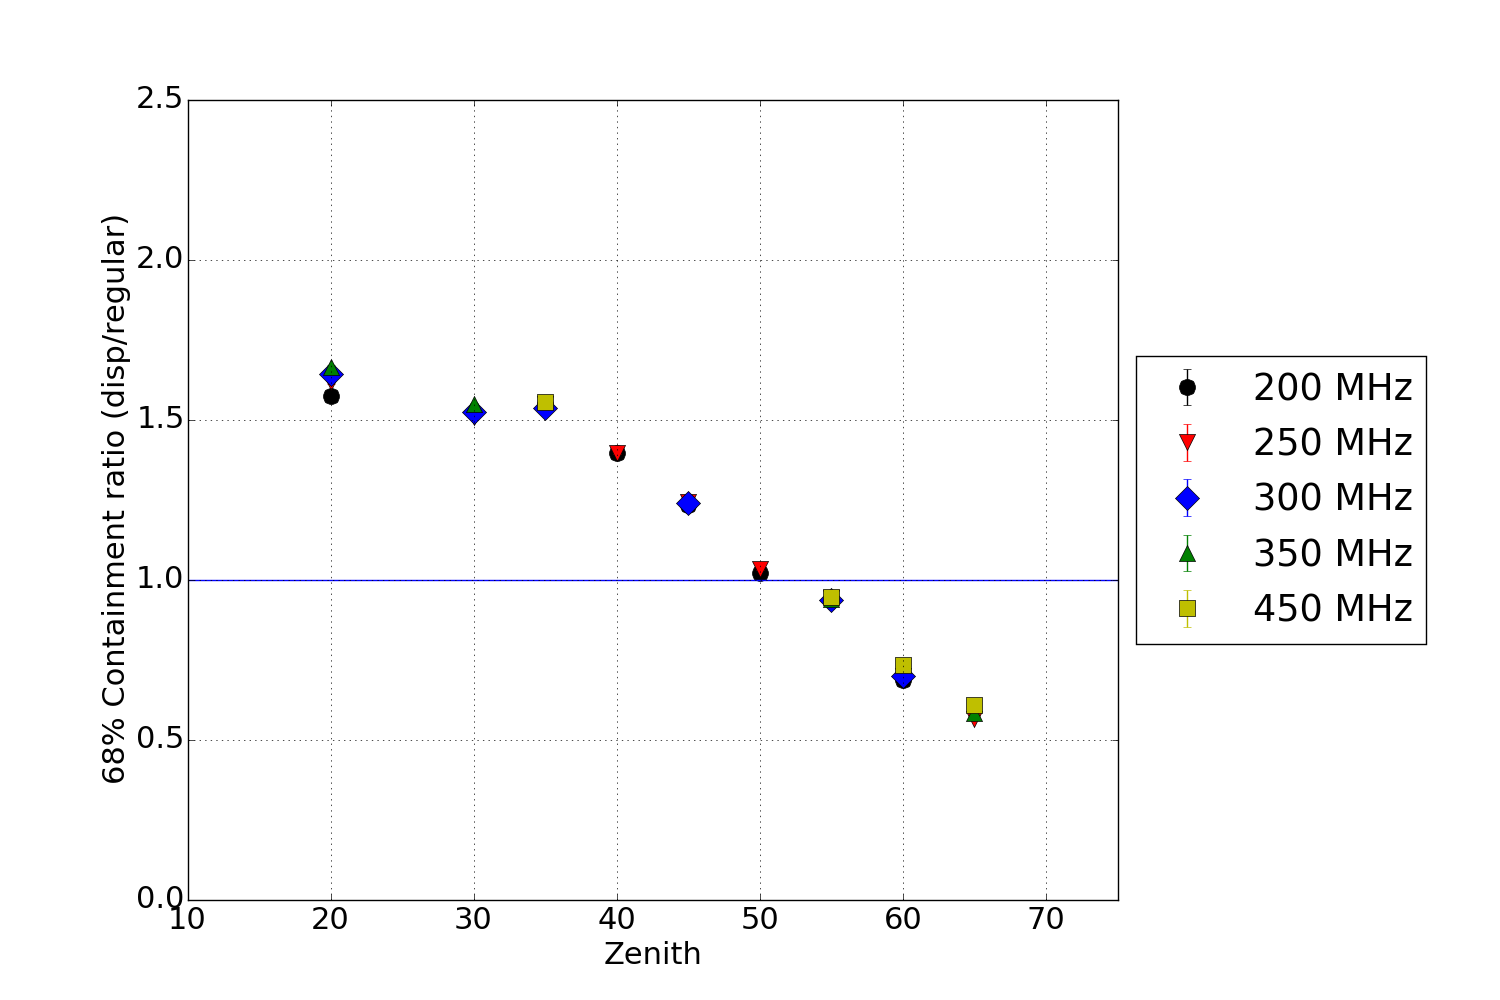
\includegraphics[width=0.8\linewidth]{images/disp_250_ratio_xzen}
  \caption[Test \disp table reconstruction (noise = $250$ MHz).]{Ratio of the \rse from reconstruction using test \disp table ($\sim 1.9\e6$ events all at noise $= 250$ MHz) and that from Method0. Note the horizontal blue line denotes the performance using Method0, so this method performs better than Method0 for zenith $>45^\circ$.}
  \label{fig:disp_ratio_250}
\end{figure}

\subsection{Over-training}
BDT based regression is quite robust under non-linear correlations between discriminating parameters, however the primary vulnerability of this method, is that  to over-training - where the decision tree starts to be informed by noise and nuisance parameters in the training sample rather than relevant effects. This results in substantially different reconstruction efficiencies between training and testing samples. The ROOT TMVA package has a built-in test for over-training where it randomly selects a given fraction of the supplied events (for the purposes of this work, this fraction was taken to be 50\%) to use for testing. These events are then not used to train the regression trees and are instead used only to generate a measure of the over-training.
This check of the over-training for one of the test tables (noise $= 450$ MHz), shown in Fig. \ref{fig:overtraining}, demonstrates that there was no meaningful over-training of the table at least based on effects in the training sample.

There remains however, the possibility of effects related to noise level that might appear in the training \textit{and} testing samples (which are generated separately at each noise level), but not in observational data sets, which would be overlooked by this measure of over-training.

\begin{figure}[H]
  \centering
  \subfigure[Deviation of reconstructed \disp parameter from Monte-Carlo \disp parameter in training sample.]{
    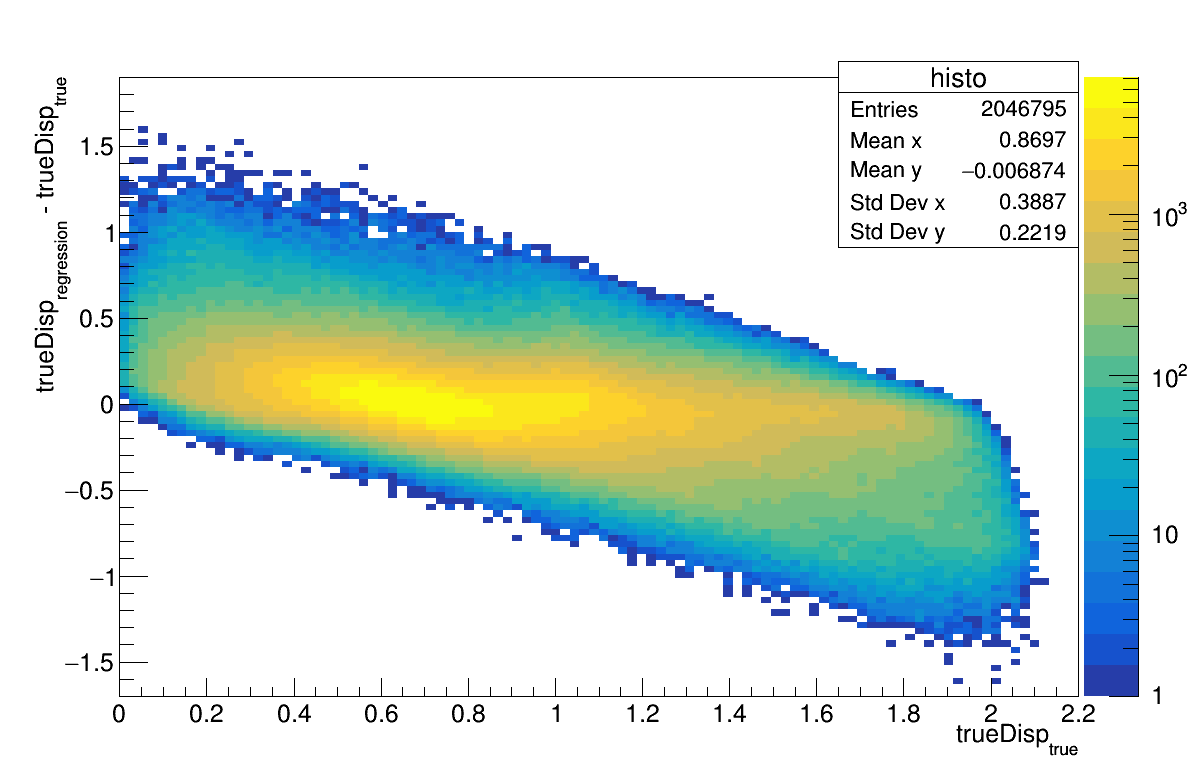
\includegraphics[width=.47\linewidth]{images/trueDisp_Train}
    \label{fig:disp_train_overtraining}
  }
  \subfigure[Deviation of reconstructed \disp parameter from Monte-Carlo \disp parameter in testing sample.]{
    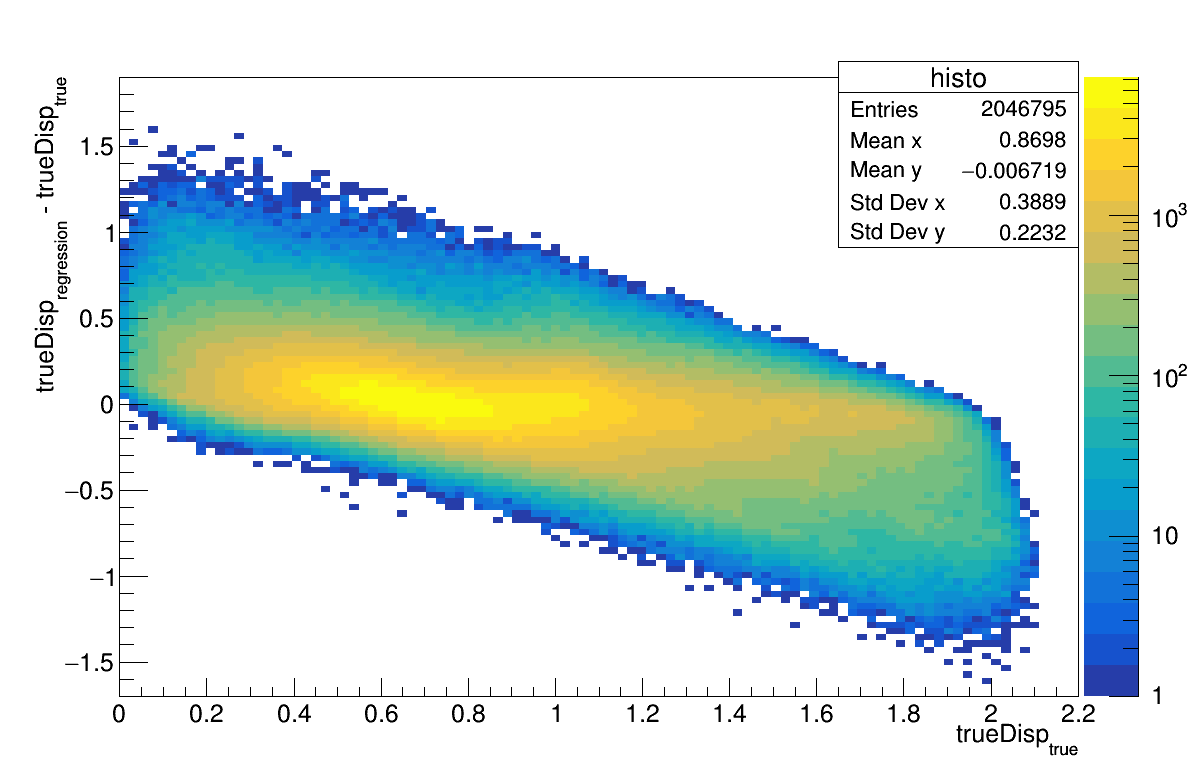
\includegraphics[width=.47\linewidth]{images/trueDisp_Test}
    \label{fig:disp_test_overtraining}
  }
  \subfigure[Deviation of reconstructed \disp Error parameter from Monte-Carlo \disp Error parameter in training sample.]{
    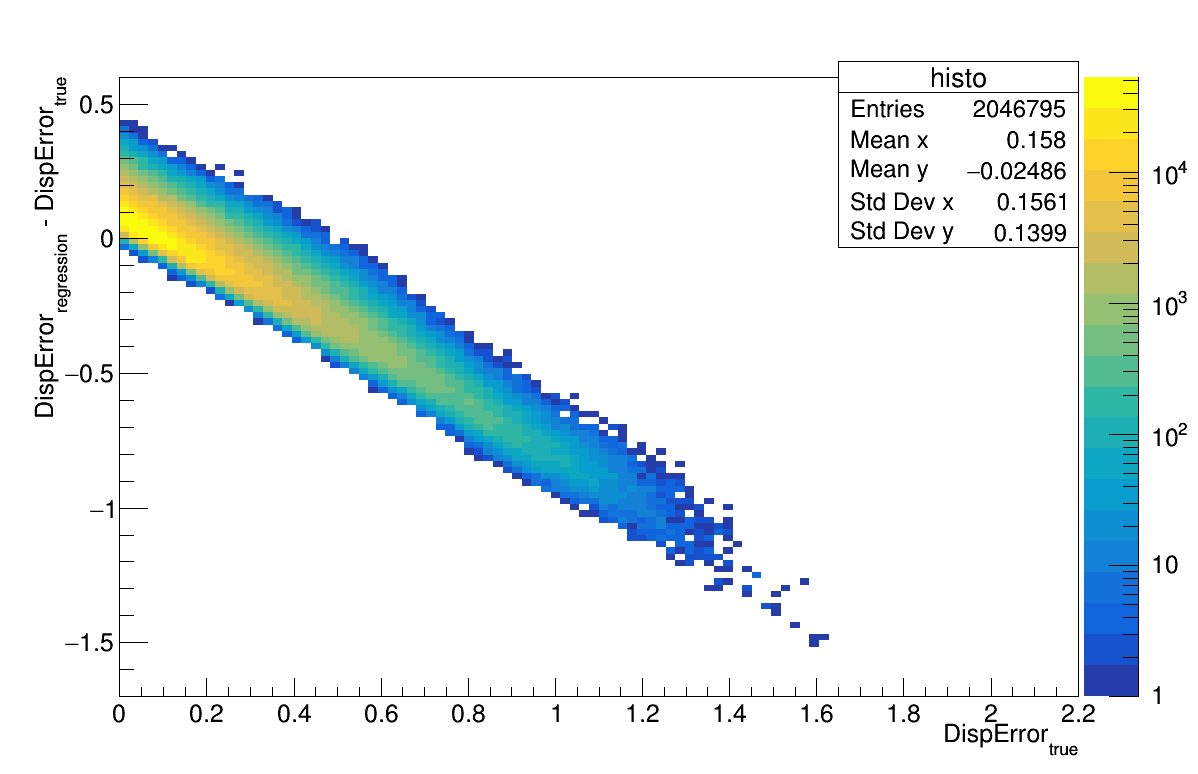
\includegraphics[width=.47\linewidth]{images/DispError_Train}
    \label{fig:dispErr_train_overtraining}
  }
  \subfigure[Deviation of reconstructed \disp Error parameter from Monte-Carlo \disp Error parameter in testing sample.]{
    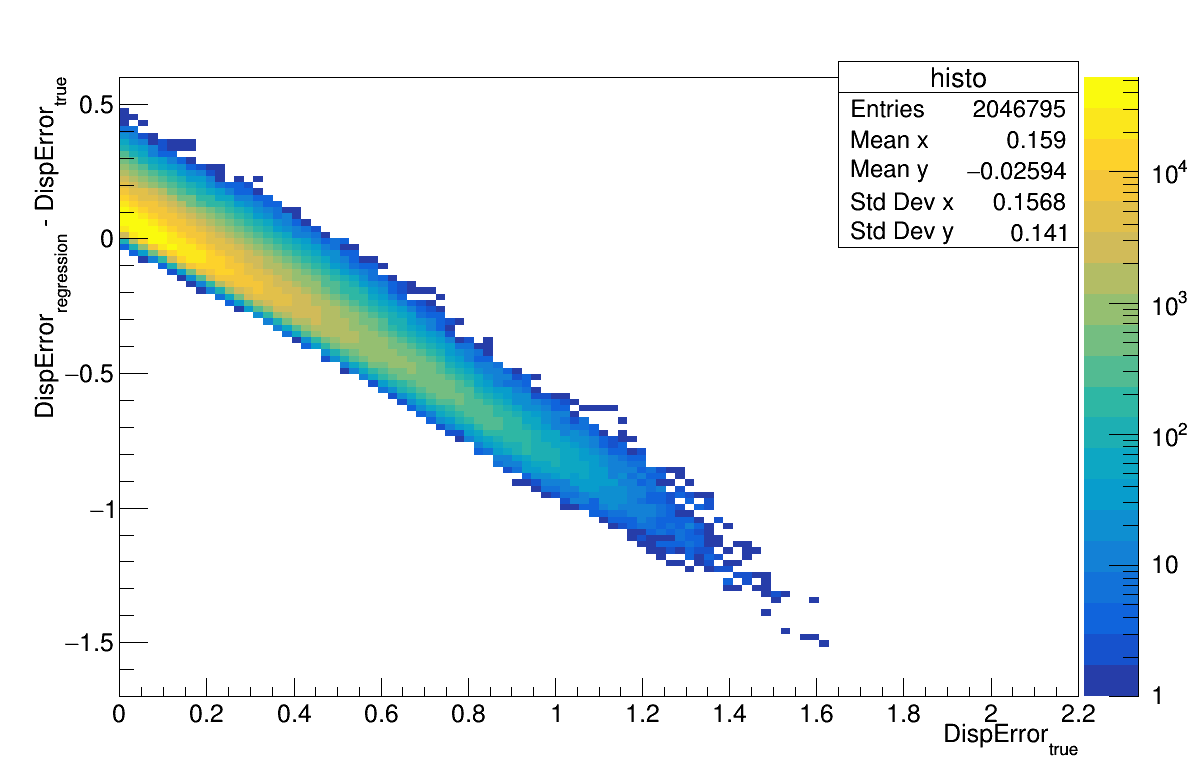
\includegraphics[width=.47\linewidth]{images/DispError_Test}
    \label{fig:dispErr_test_overtraining}
  }
  \subfigure[Deviation of reconstructed MAError parameter from Monte-Carlo MAError parameter in training sample.]{
    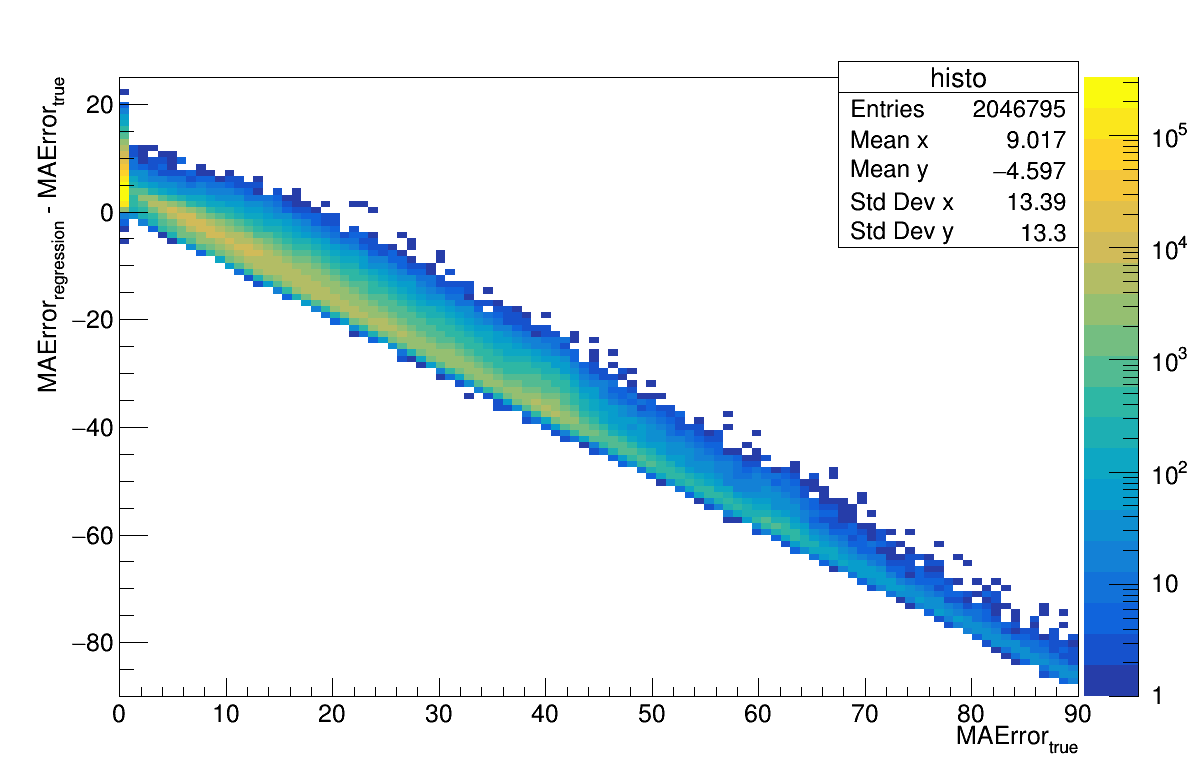
\includegraphics[width=.47\linewidth]{images/MAError_Train}
    \label{fig:MAErr_train_overtraining}
  }
  \subfigure[Deviation of reconstructed MAError parameter from Monte-Carlo MAError parameter in testing sample.]{
    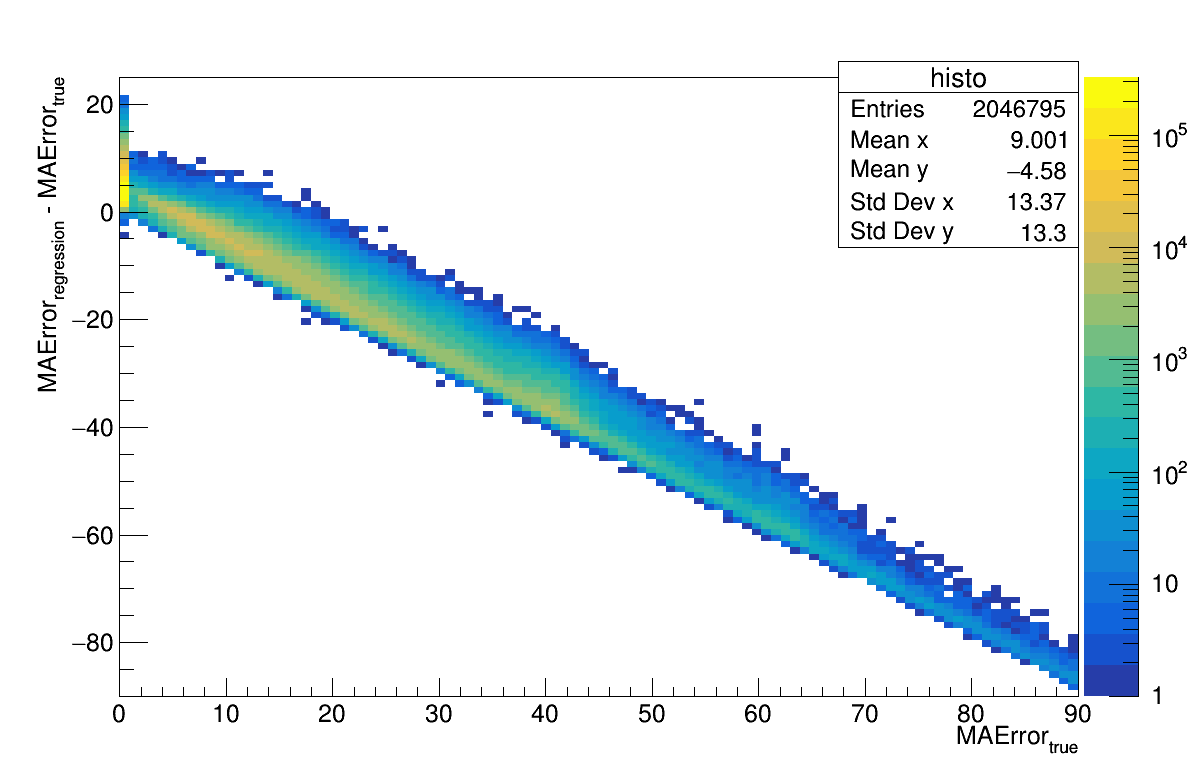
\includegraphics[width=.47\linewidth]{images/MAError_Test}
    \label{fig:MAErr_test_overtraining}
  }
  \caption[Over-training test.]{Over-training check on reconstruction using a \disp table generated at a single noise level. The left column shows the deviation of the reconstructed parameter from the true value in the training sample and the column on the right shows the same in the testing sample. The difference between the two columns is small which suggests there is little or no overtraining.}
  \label{fig:overtraining}
\end{figure}

\subsection{Noise Related Effects}
The first set of \disp tables was also generated at a single noise level ($250$ MHz), allowing us to test the dependence of the resolution of this method (as measured by R$_{68}$) on noise level -- some kind of noise-dependent effect would suggest over-training that would not be evident from the testing sample in the ROOT TMVA method since all the data provided to the package would have been at the same noise level. A comparison of angular resolution across noise levels revealed no significant dependence of the \rse on noise (see Fig. \ref{fig:olddisp_ratio}, \ref{fig:disp_ratio_250} and \ref{fig:disp_ratio_450}).

\begin{figure}[htbp]
  \centering
  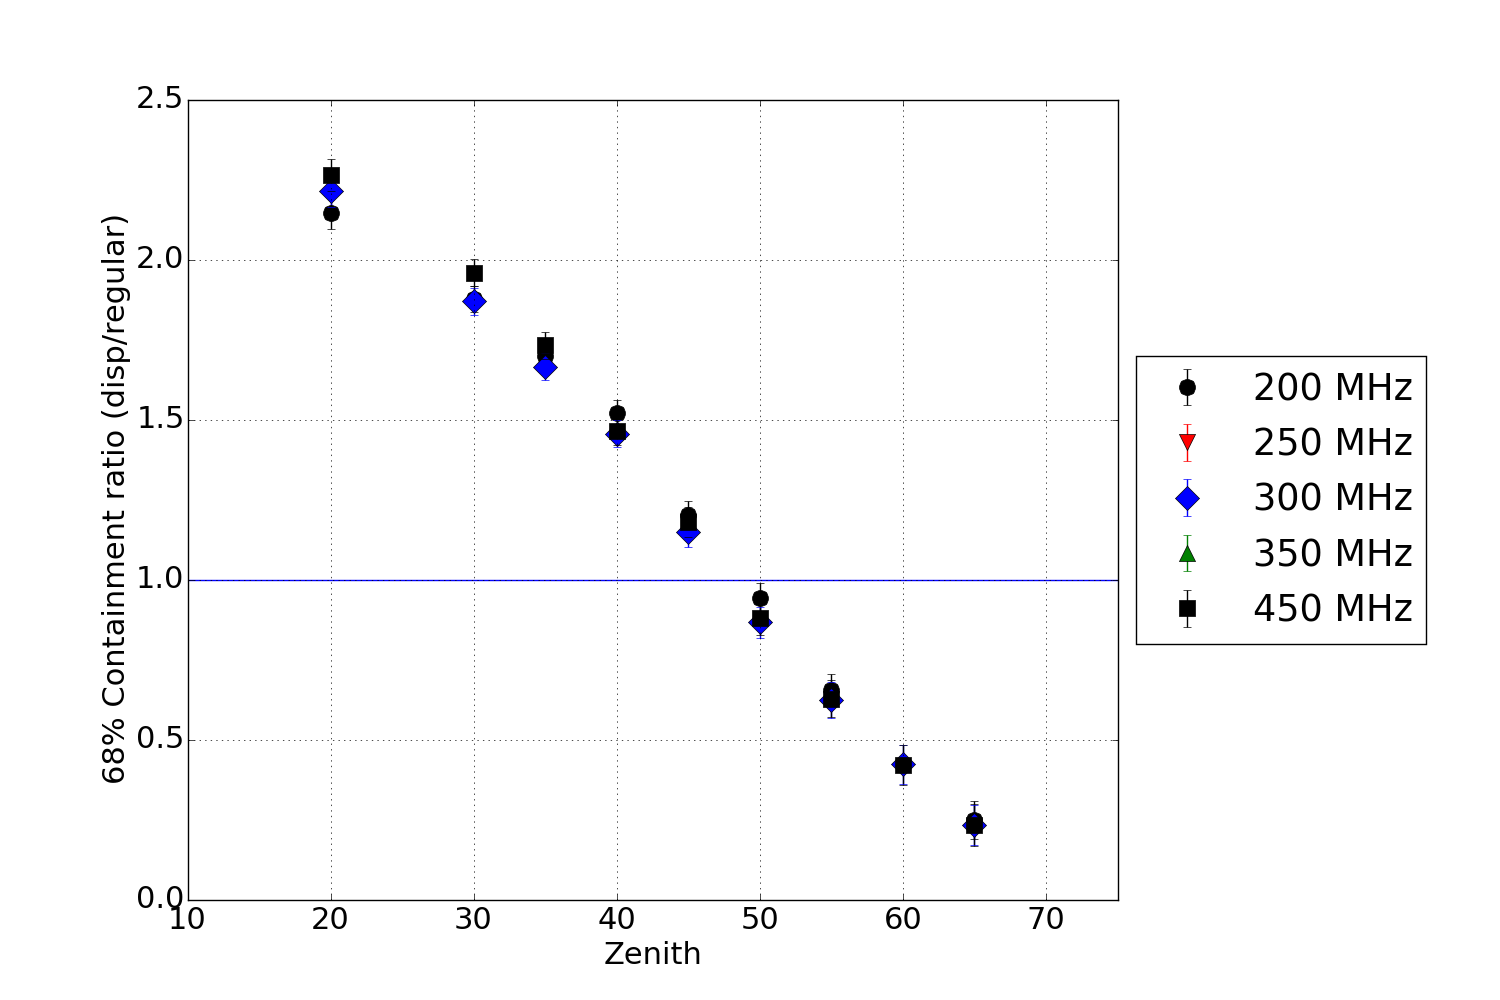
\includegraphics[width=0.8\linewidth]{images/disp_450_ratio_xzen}
  \caption[\disp table reconstruction vs noise.]{Ratio of \rse of the noise=450MHz \disp table ($\sim 2.1\e6$ events) to that from Method0.}
  \label{fig:disp_ratio_450}
\end{figure}

A second set of test \disp tables was generated using a single noise level (noise $= 450$ MHz) to test for noise-related over-training (see Fig. \ref{fig:disp_ratio_450}). These tables performed slightly better than the first test tables and comparably to the standard \disp tables. Since the noise-related effects did not seem to play a significant role in reconstruction, noise was dropped as a discriminating parameter for further analysis.

To generate a set of \disp tables with better angular resolution (as measured by \rse\hspace{-4pt}), another set of \disp tables was trained on a larger number of simulations across zenith angles (as before) as well as across the noise spectrum.

\subsection{Higher Statistics Tables}
Once it was determined that there was no significant over-training in the small sample \disp tables, and the noise level had little bearing on the \rse measure of the reconstruction, it was determined that different noise level simulation events could be used as independent training events to have a higher statistics \disp table, and make small improvements on the statistical uncertainty on the reconstruction. The simulation data from across the noise spectrum and zenith range was used to generate a \disp table that sampled the entire parameter space more exhaustively.

A new set of \disp tables was generated (Fig. \ref{fig:disp_ratio_450x4}) with a training sample four times that of the initial test tables. The improvements in resolution due to change in sample size were modest, and confined to the range of zenith angles (zenith $>45^\circ$) where the standard method outperforms the \disp method quite considerably.

\begin{figure}[htbp]
  \centering
  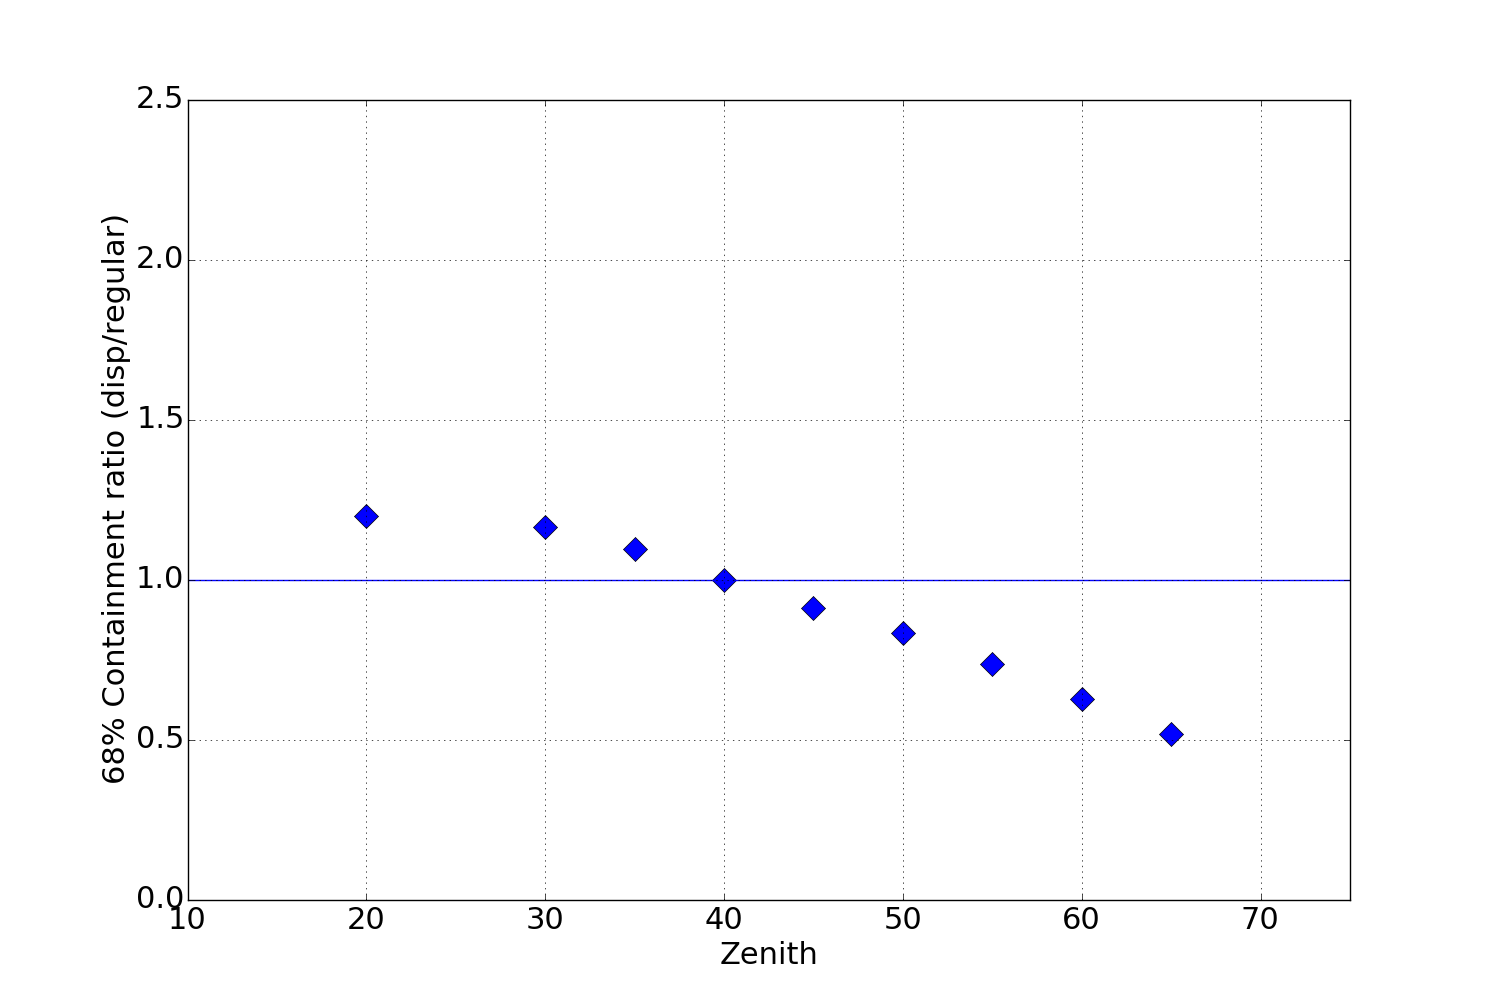
\includegraphics[width=0.8\linewidth]{images/disp_450x4size_ratio_xzen}
  \caption[Higher statistics \disp table reconstruction vs noise.]{Ratio of \rse of the noise=450MHz \disp table ($\sim 8.4\e6$ events) to that from Method0 for a higher statistics \disp table.}
  \label{fig:disp_ratio_450x4}
\end{figure}

As expected from the small statistical uncertainty on the \rse values, this increase in sample size did not lead to any meaningful improvements and a training sample of $\sim 2\e6$ was determined to be sufficient to achieve the desired resolution with small uncertainties.

\subsection{Acceptance Correction for Offset from Camera Center}
Showers arriving further from the camera center have a larger fraction of the shower arriving outside of the camera and therefore being lost. These showers are therefore reconstructed with a lower efficiency and resolution than showers arriving closer to the camera center. To compensate for this in the BDT training, so that the training sample does not mis-characterize the overabundance of events closer to the camera center as an anisotropy in incoming gamma rays, we fold in an acceptance correction by assigning a larger weight to events that are further away from the camera center.

The acceptance correction used here affects the training sample and therefore might be assumed to affect the resolution in a zenith dependent way, explaining the difference in performance between the new \disp tables and the old ones. This was tested by using a number of different correction functions in the training sample, as shown in Fig. \ref{fig:weights}

\begin{figure}[htbp]
  \centering
  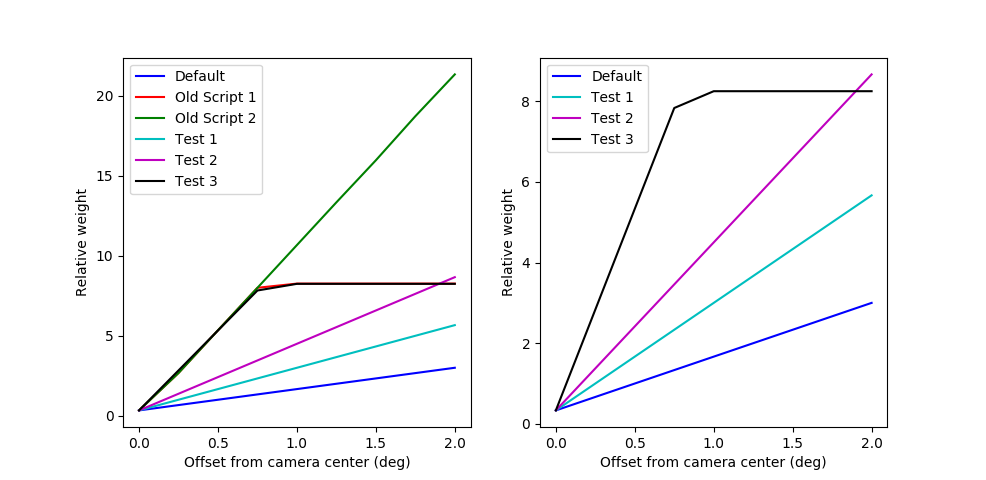
\includegraphics[width=.78\linewidth]{images/weights}
  \caption[Weight functions for offset from camera center.]{The weight functions used in the training samples in the new tables (Default, Test 1, Test 2 and Test 3) and those found in the scripts used to generate the older tables (Old Script 1, Old Script 2).}
  \label{fig:weights}
\end{figure}

These tests reveal small changes in the \rse value despite large changes in the correction function (Fig. \ref{fig:weight_tests}). This suggests that the \disp tables are not sensitive to changes in acceptance and therefore the different acceptance functions are unlikely to be the reason why the new \disp tables perform worse at smaller zenith angles.

\begin{figure}[htbp]
  \centering

  \subfigure[Camera offset acceptance correction default.]{
    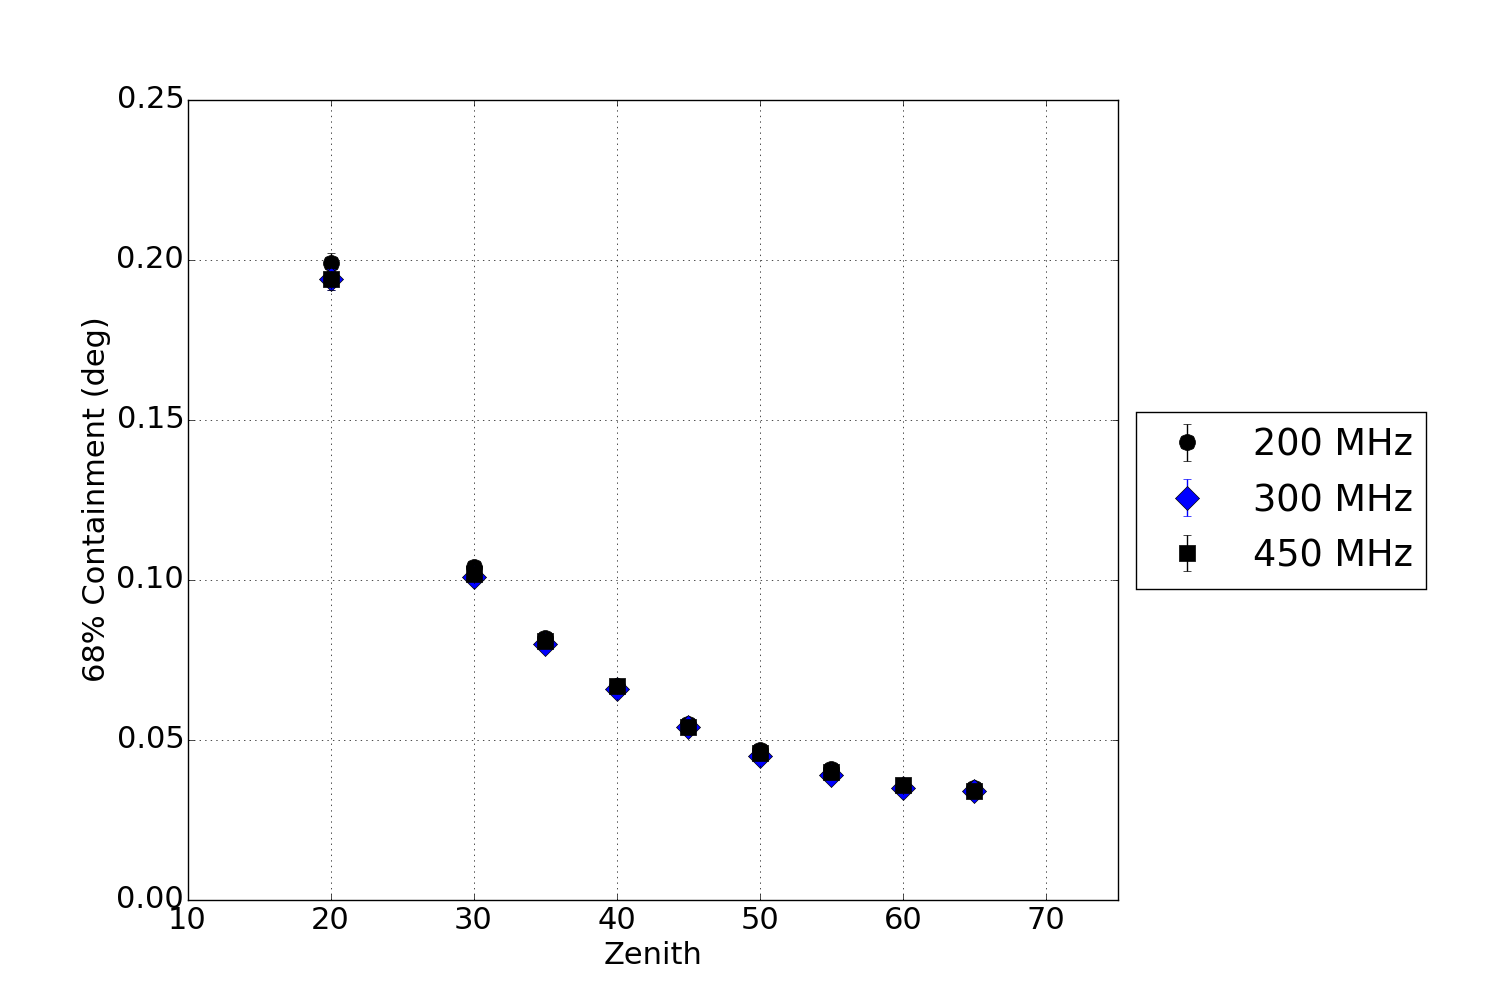
\includegraphics[width=.45\linewidth]{images/disp_450size_val_xzen}
    \label{fig:weight_test_default}}
  \subfigure[Camera offset acceptance correction test 1.]{
    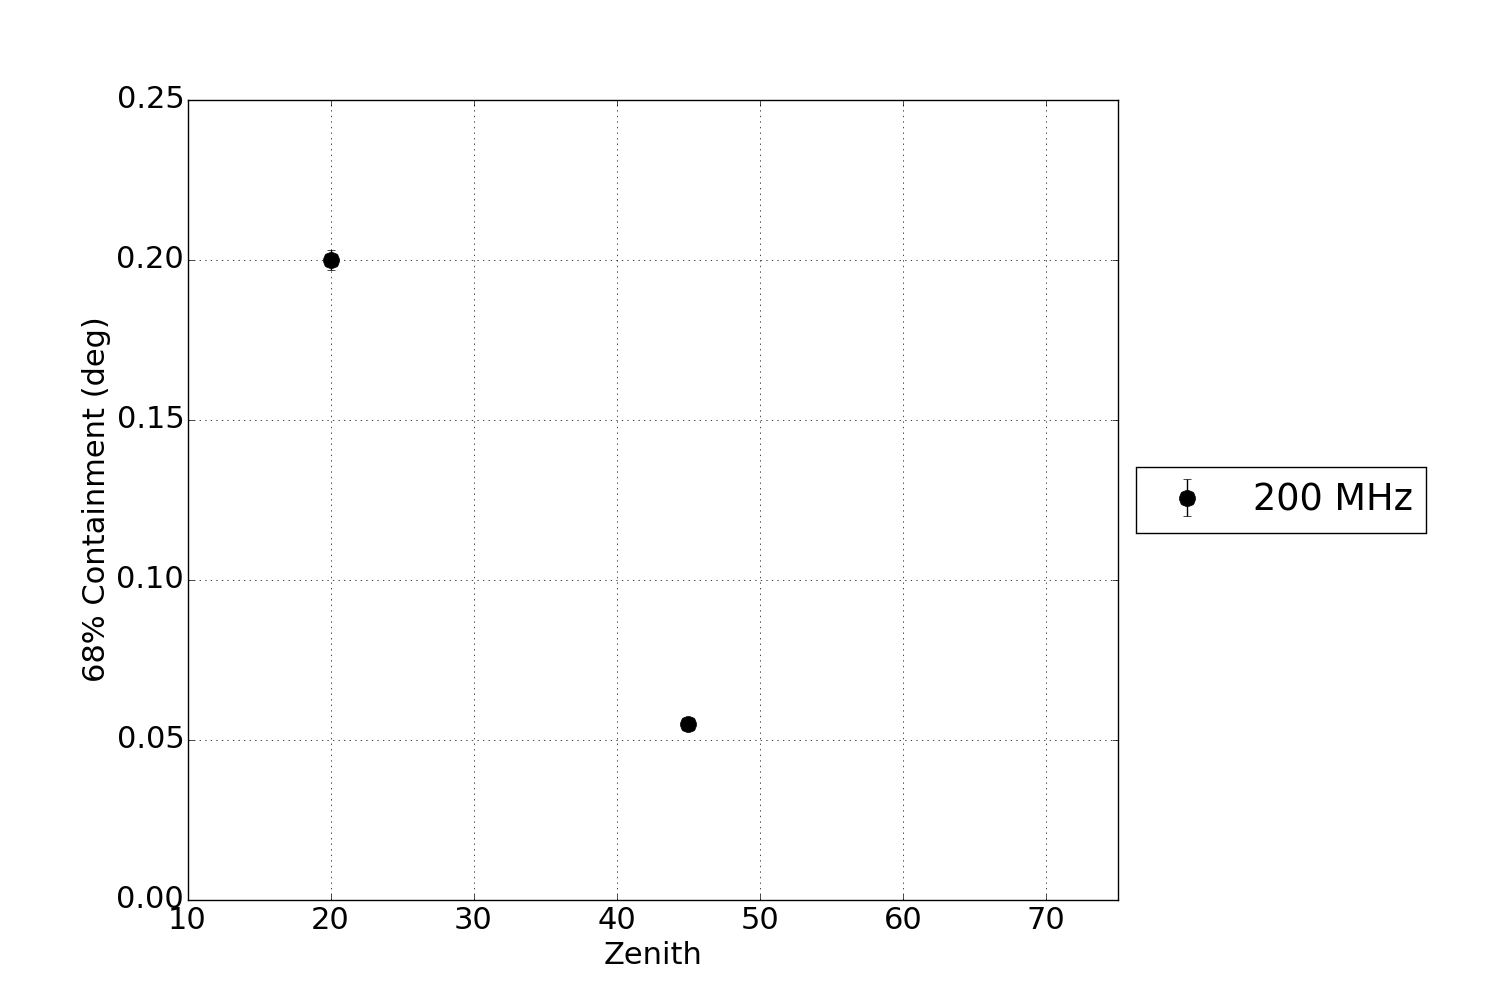
\includegraphics[width=.45\linewidth]{images/disp_450size_wtfix_val_xzen}
    \label{fig:weight_test_1}}
  \subfigure[Camera offset acceptance correction test 2.]{
    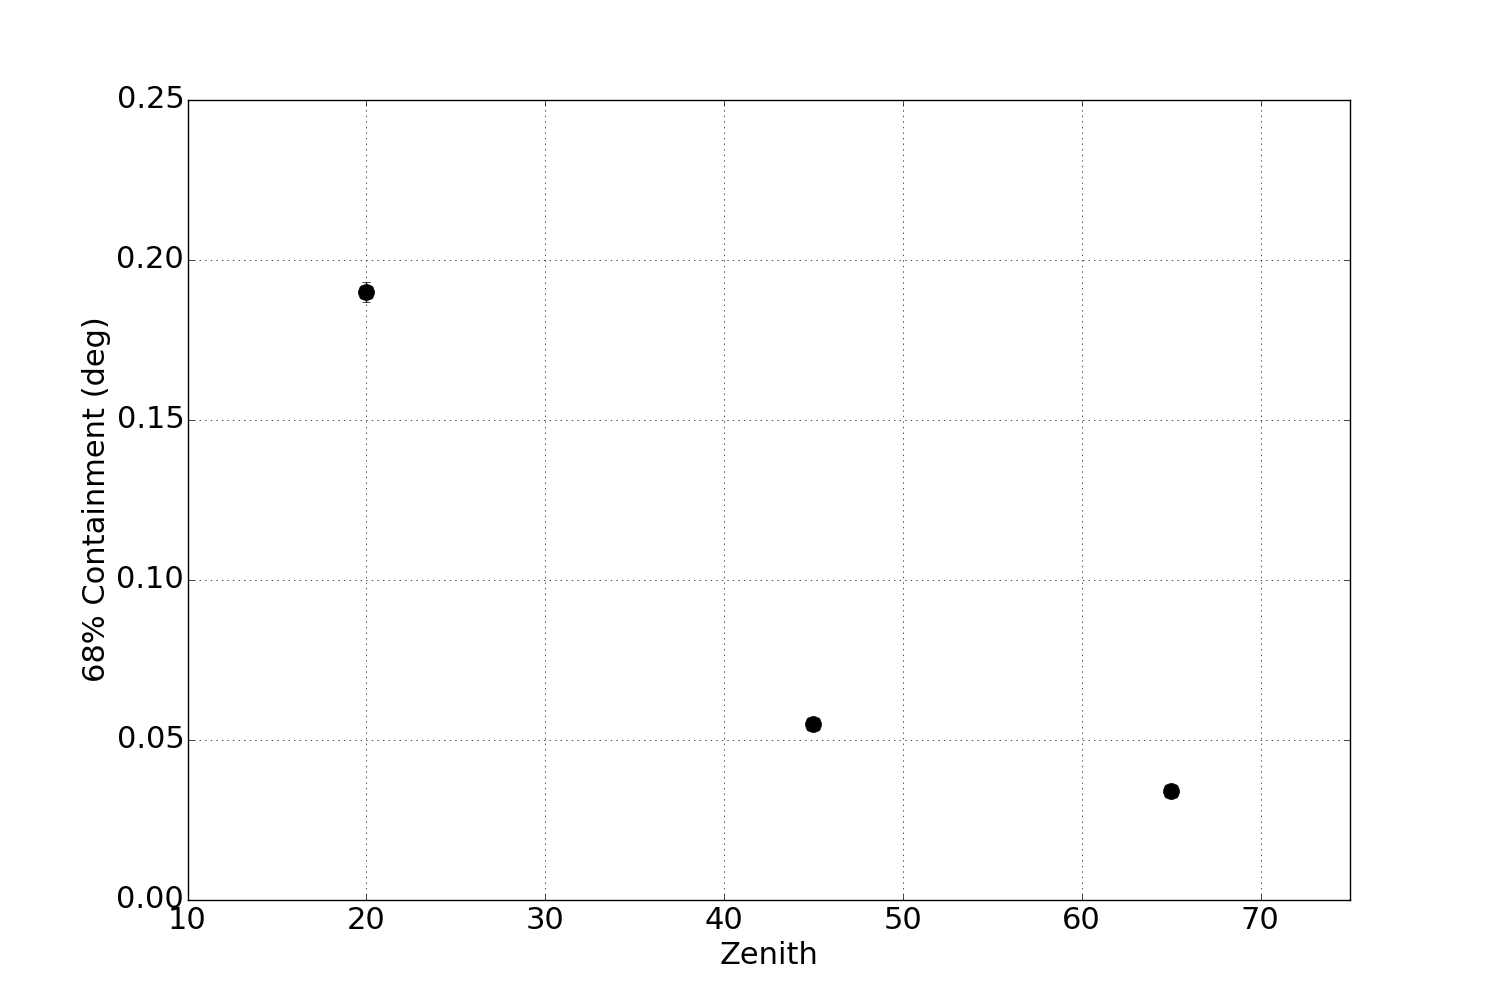
\includegraphics[width=.45\linewidth]{images/disp_450x4size_wtfix_val_xzen}
    \label{fig:weight_test_2}}
  \subfigure[Camera offset acceptance correction test 3.]{
    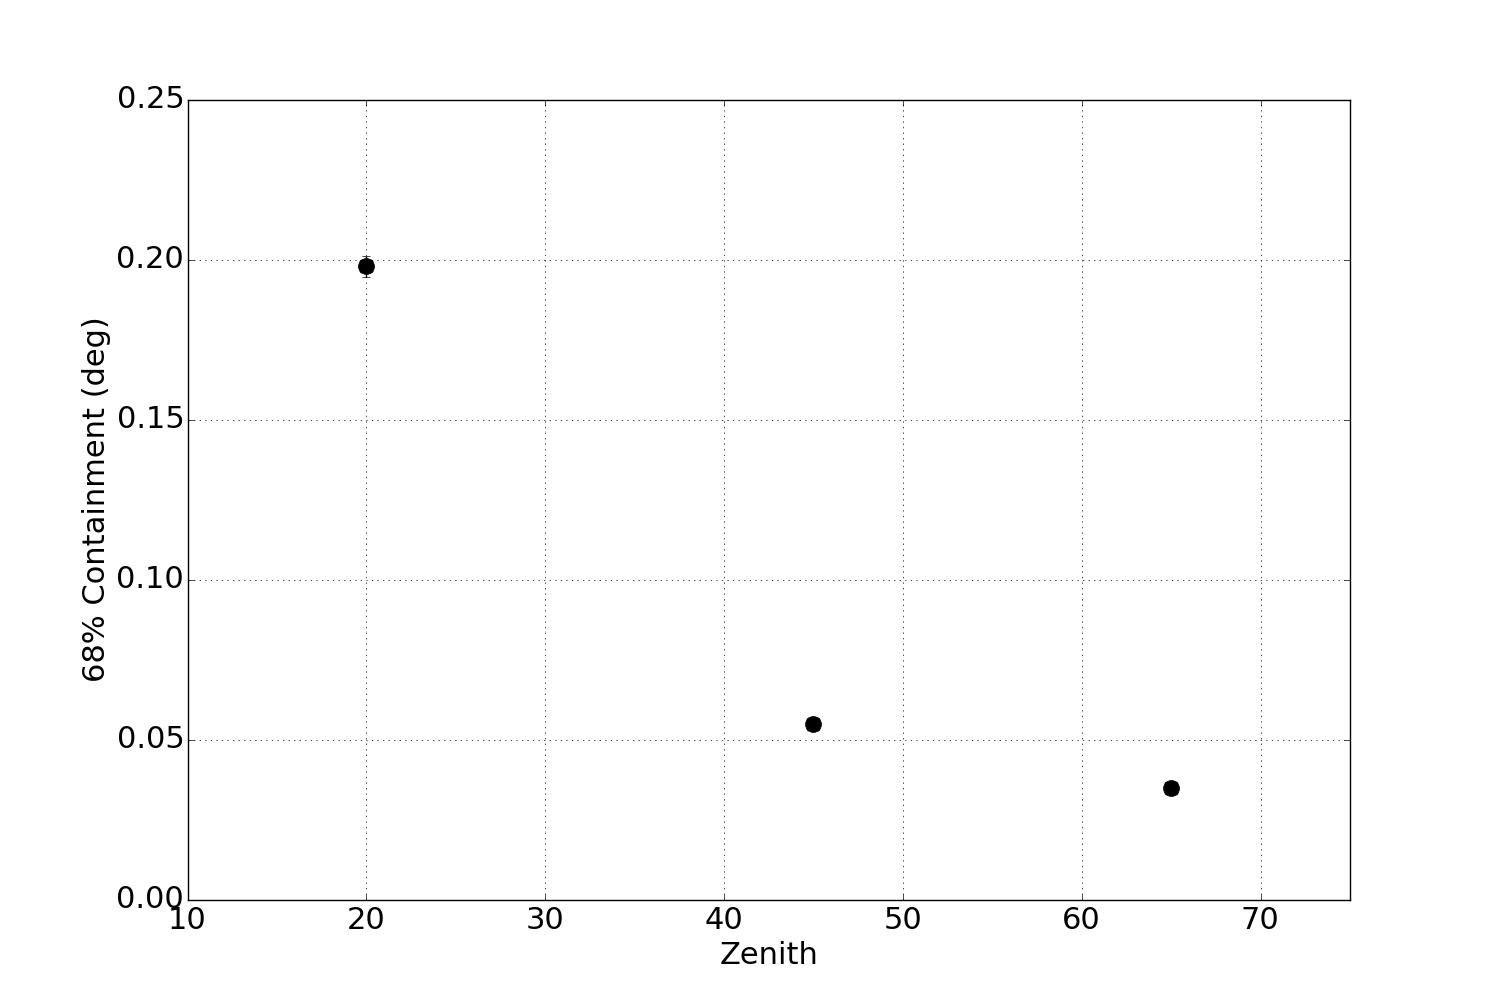
\includegraphics[width=.45\linewidth]{images/disp_broken_wtfix_val_xzen}
    \label{fig:weight_test_3}}

  \caption[\rse for the acceptance correction functions.]{\rse for each acceptance correction function shown in Fig. \ref{fig:weights}. The changes in acceptance correction do not meaningfully change the \rse for the reconstruction.}
  \label{fig:weight_tests}
\end{figure}

\subsection{Energy Dependence}
Another important dependence of the reconstruction resolution (and therefore the \rse\hspace{-4pt}) is that on energy. Higher energy photons are expected to comprise a large fraction of LZA photons which have to travel longer through the atmosphere and therefore must remain above the threshold energy deeper into the atmosphere. Conversely, high energy photons are expected to make up a small fraction of SZA photons (and more generally, all cosmic photons) due to the relative overabundance of generating processes as well as the greater relative likelihood of down-scattering than up-scattering. A much better resolution at higher energy would also be expected to contribute to the improved resolution at LZA.

\begin{figure}[htbp]
  \centering
  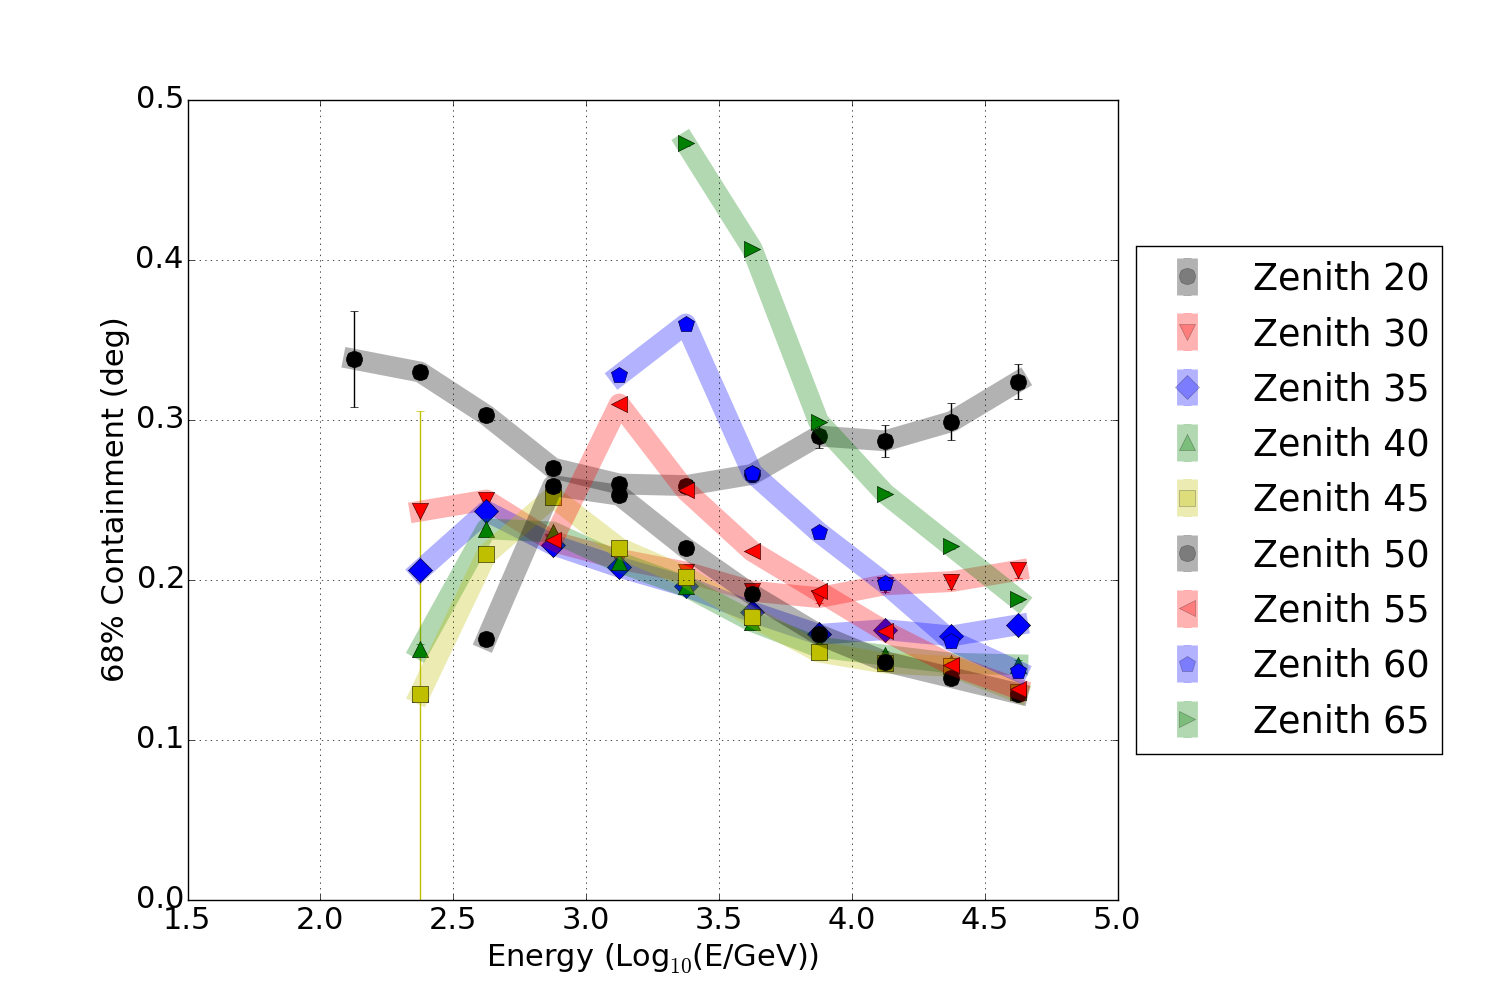
\includegraphics[width=.9\linewidth]{images/reg_energy}
  \caption{Energy Dependence of Method0.}
  \label{fig:energy_reg}
\end{figure}

\begin{figure}[htbp]
  \centering
  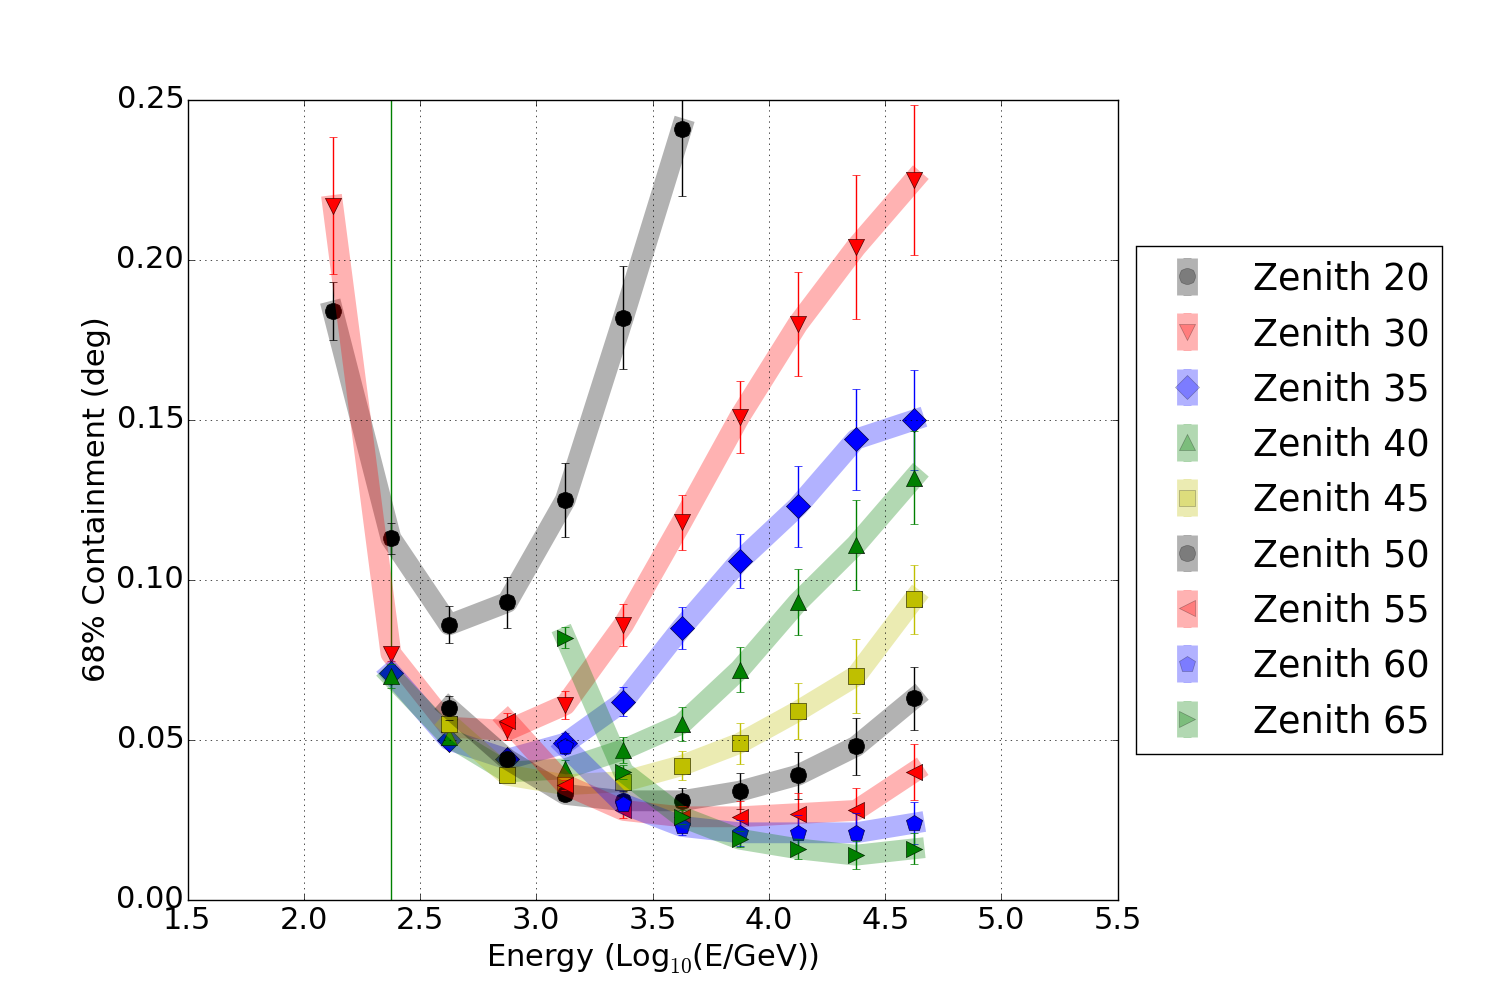
\includegraphics[width=.9\linewidth]{images/disp_standard_energy}
  \caption{Energy Dependence of the old Method5t.}
  \label{fig:energy_disp_standard}    
\end{figure}

\begin{figure}[htbp]
  \centering
  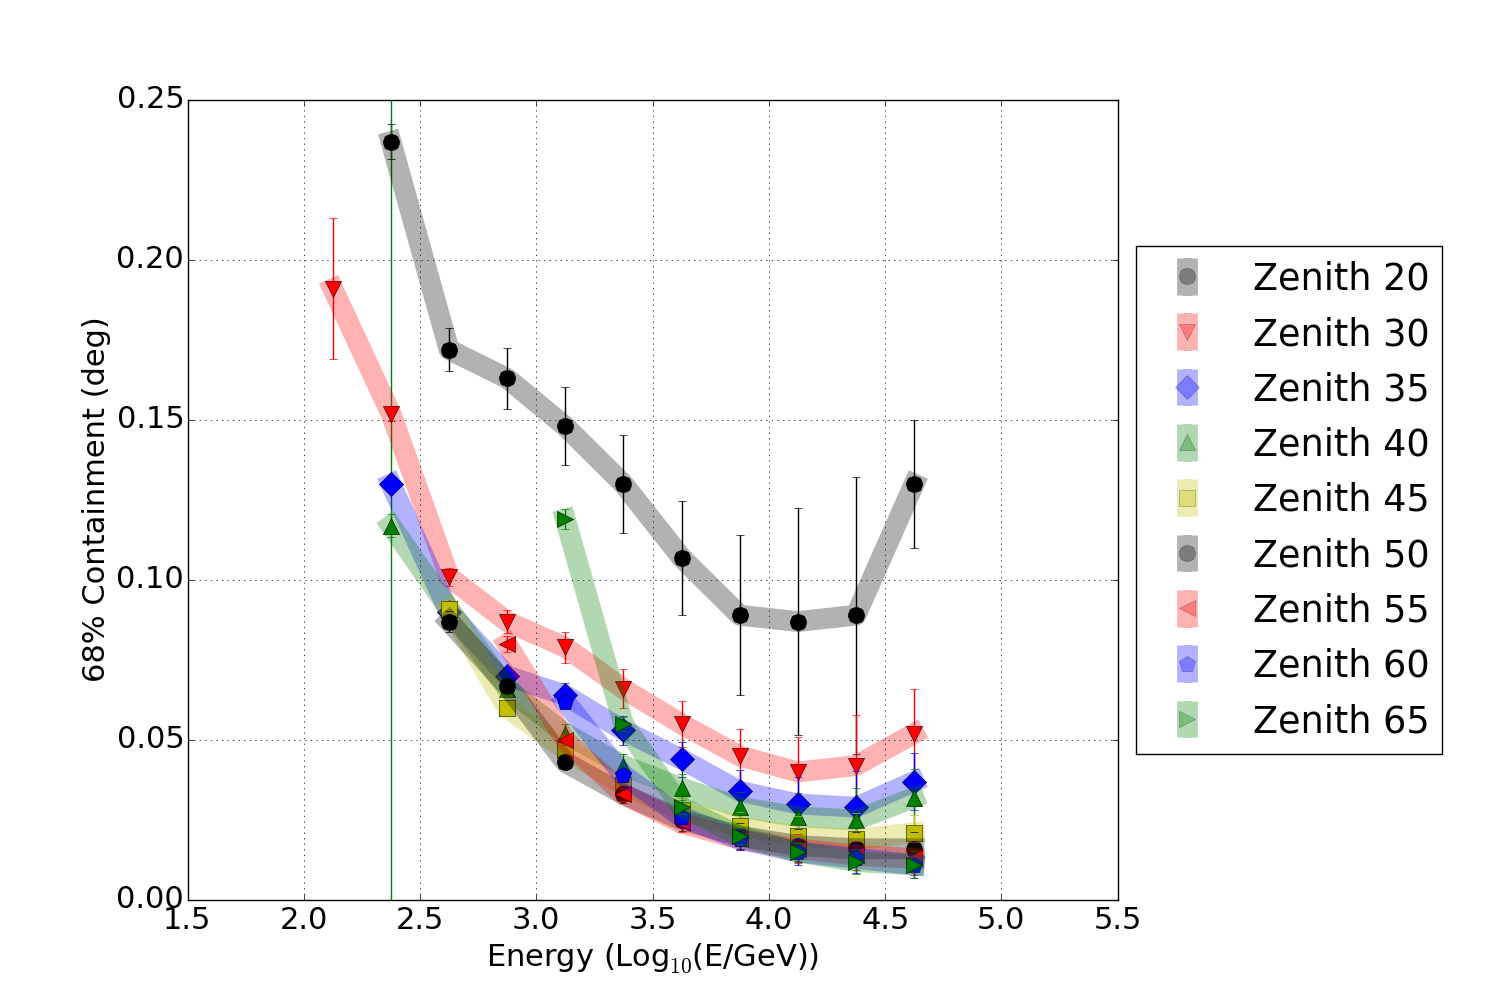
\includegraphics[width=.9\linewidth]{images/disp_450_energy}
  \caption{Energy Dependence of the new Method5t.}
  \label{fig:energy_disp_450}    
\end{figure}

The Method0 energy dependence (Fig. \ref{fig:energy_reg}) follows the same trend as in Fig. \ref{fig:disp_res}. The energy dependence for the older \disp tables (Fig. \ref{fig:energy_disp_standard}) appears to have a minimum in \rse close to 1 TeV and performs worse at lower \textit{and} higher energies, though there is large variation with zenith angle. The energy dependence for the newer \disp tables (Fig. \ref{fig:energy_disp_450}) on the other hand appears to do better at higher energies for all zenith angles. At energies above $\sim 2.37$ TeV and zenith angle greater than $30^\circ$, the \rse is at or better than $0.075^\circ$ (see Fig. \ref{fig:energy_new_contour}).

\begin{figure}[htbp]
  \centering
  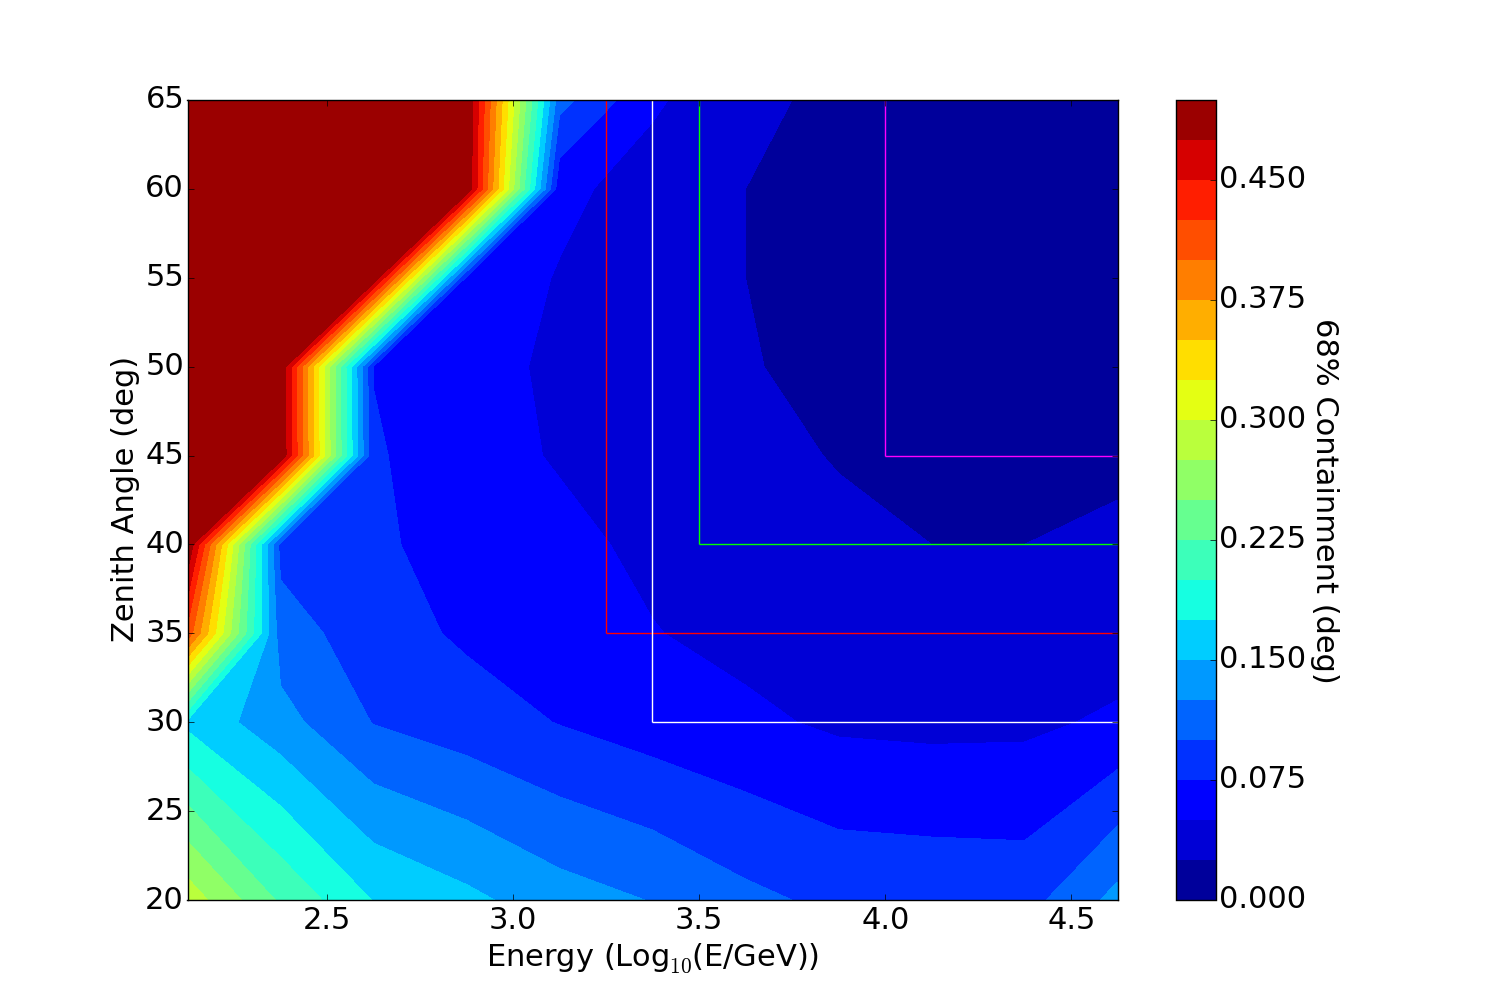
\includegraphics[width=.9\linewidth]{images/disp_450x4size_contour}
  \caption[Energy and zenith dependence of the new Method5t.]{Energy and zenith dependence of the new Method5t, with contours for \rse at intervals of $0.025^\circ$ up to $0.5^\circ$. The upper-left corner shows a sharp drop in resolution in the large-zenith low-energy region, this is due to low statistics. The boxed regions show regions of minimum resolution as described in table \ref{tab:res_energy}}
  \label{fig:energy_new_contour}
\end{figure}

\begin{figure}[htbp]
  \centering
  \subfigure{
    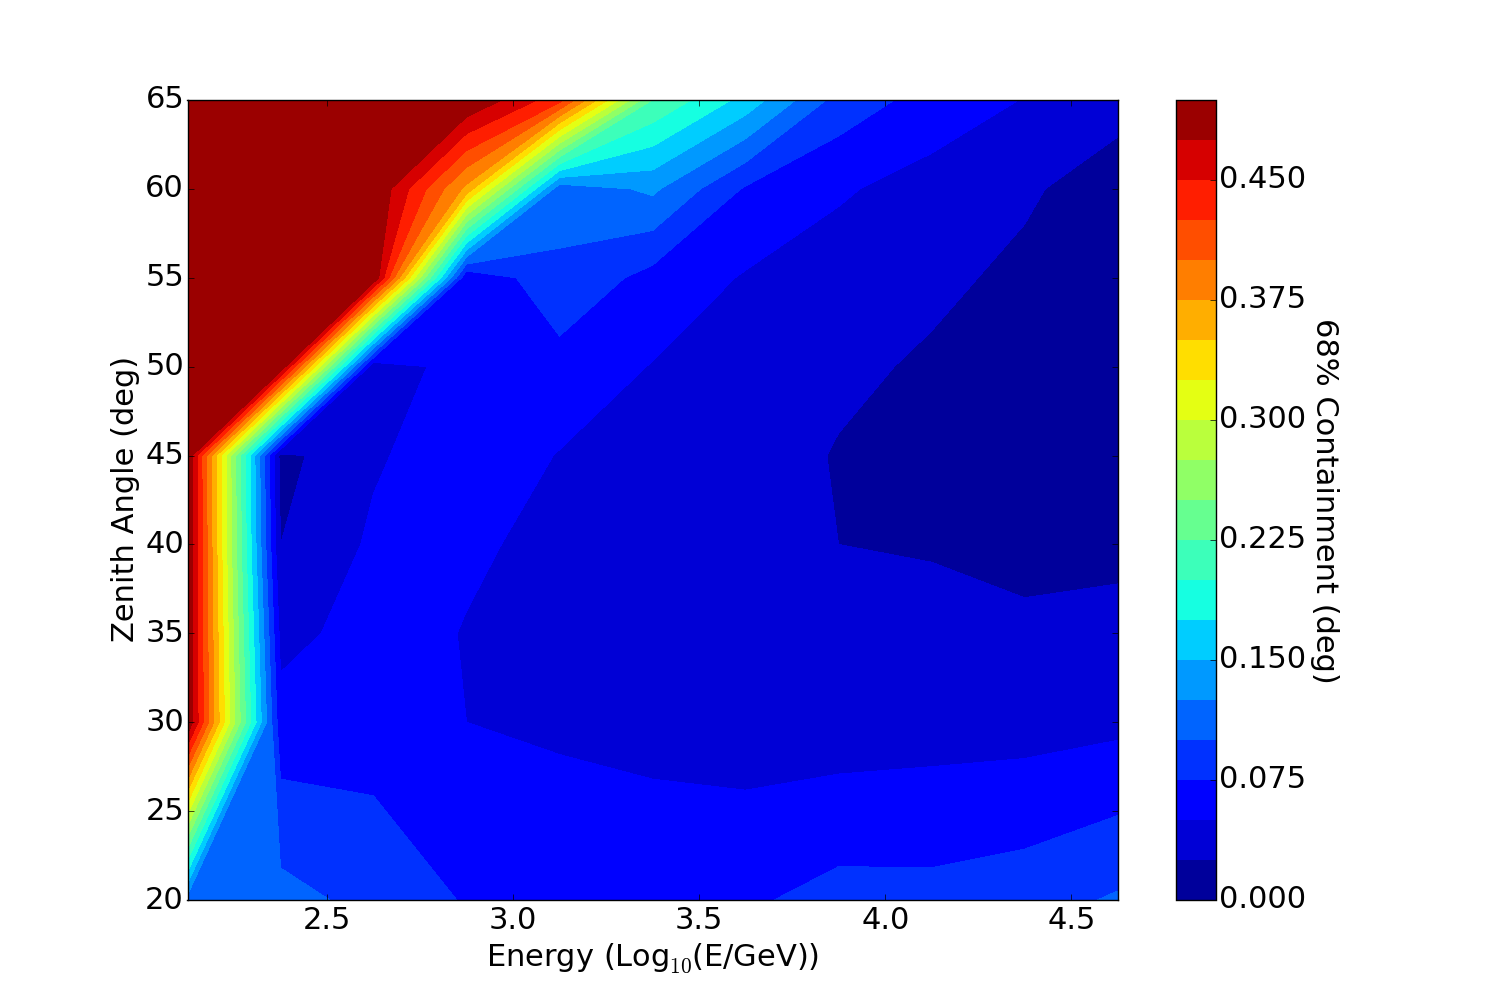
\includegraphics[width=0.47\linewidth]{images/reg_contour}
  }
  \subfigure{
    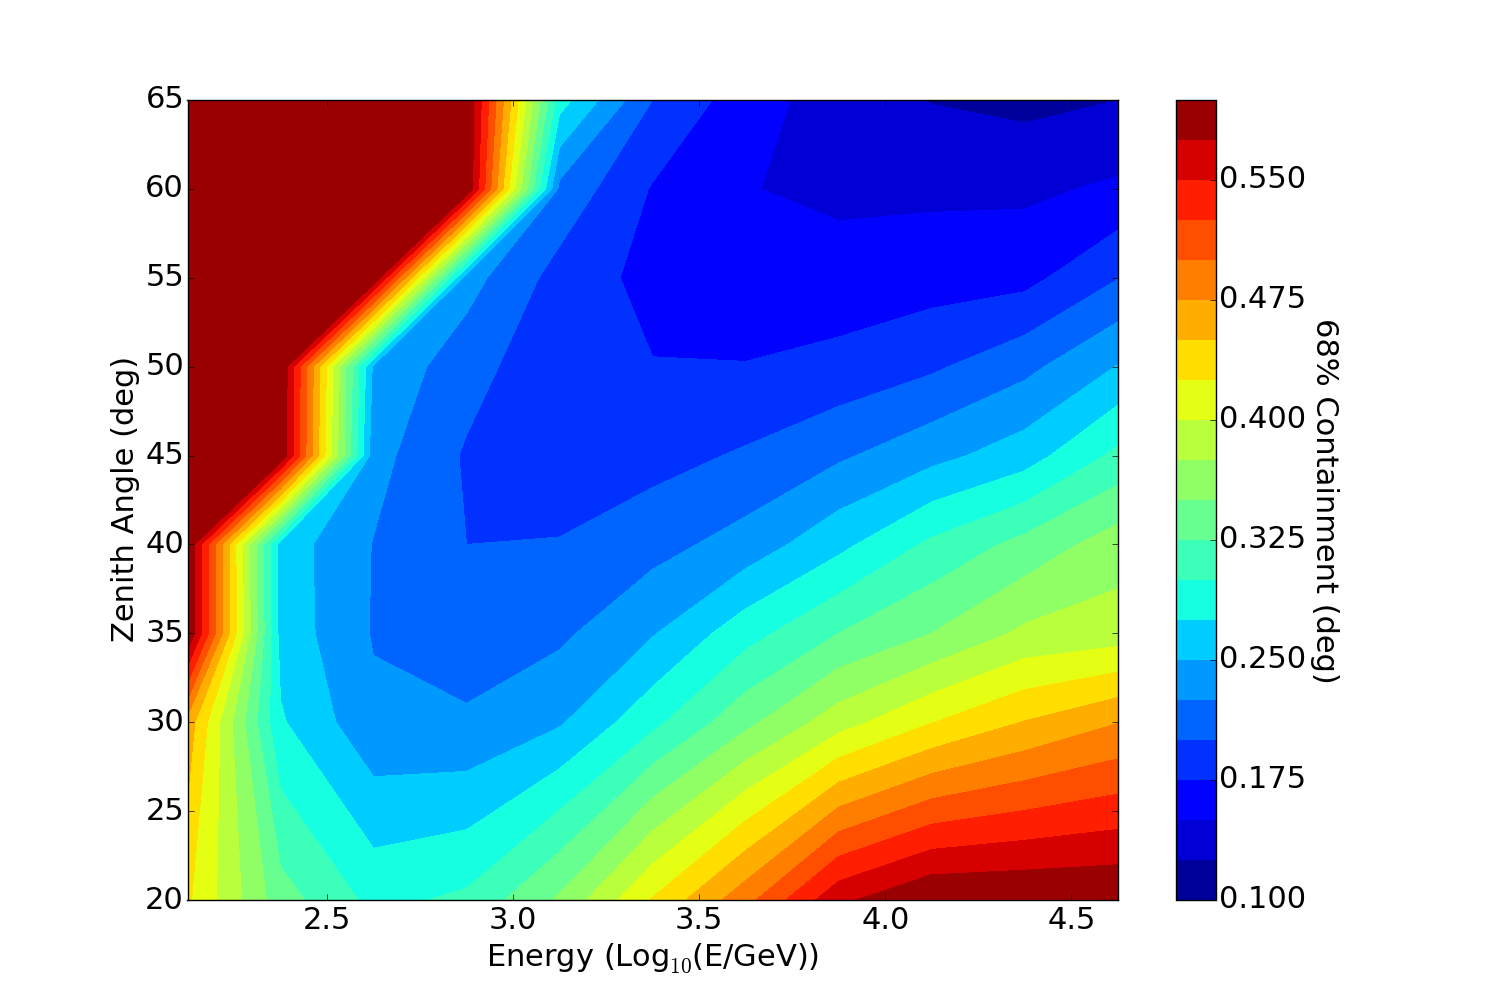
\includegraphics[width=0.47\linewidth]{images/disp_standard_contour}
  }
  \caption[Energy and zenith dependence of Method0 and the old Method5t]{Energy and zenith dependence of the geometric reconstruction (left) and the old Method5t (right), with contours for \rse at intervals of $0.025^\circ$ up to $0.5^\circ$. The range of usefulness for Method5t (relative to Method0) now extends to $E>1$TeV and $\phi>55^\circ$.}
  \label{fig:energy_contour}
\end{figure}

\begin{table}[htbp]
  \begin{center}
    \begin{tabularx}{0.85\textwidth}{ X | X | X | X }
      \hline
      \textbf{Min. Zenith (deg)} & \textbf{Min. Energy (TeV)} & \textbf{Min. Energy (Log$_{10}$(E/GeV))} & \textbf{\rse (deg)} \\
      \hline\hline
      45 & 10.0 & 4.0 & 0.025 \\
      40 & 3.16 & 3.5 & 0.05 \\
      35 & 1.78 & 3.25 & 0.075 \\
      30 & 2.37 & 3.375 & 0.075 \\
    \end{tabularx}
    \caption[\rse for simulations with energy and zenith.]{\rse for simulations with energy and zenith as shown in Fig. \ref{fig:energy_new_contour}\label{tab:res_energy}.}
  \end{center}
\end{table}
Because the best resolution contours strongly constrain the parameter space to regions where statistics are low, constraints were used that were not simple rectangles. Instead an effective lower Reimann sum was used to construct an approximation that maximized the usable parameter space while imposing the most conservative constraints on parameter space between the simulated zenith values. The resulting contours are shown in Fig. \ref{fig:contour_boxplot}. These can be denoted as the sums of rectangles as shown in table \ref{tab:contour_boxplot}
% \begin{table}[htbp]
%   \begin{center}
%     \begin{tabularx}{0.85\textwidth}{ X | X | X | X }
%       \hline
%       & \textbf{Zenith range (deg)} & \textbf{Energy (Log$_{10}$(E/GeV))} & \textbf{\rse (deg)} \\
%       \hline\hline
%       % \res = 0.025
%       % (fEnergyGeV>TMath::Power(10.0, 3.875) && ZenithDeg>
%       1. & $>45$ & $>3.75$ & 0.025 \\
%       \hline
%       % \res = 0.03
%       % (fEnergyGeV>TMath::Power(10.0, 3.875) && ZenithDeg>40) ||
%       % (fEnergyGeV>TMath::Power(10.0, 3.625) && ZenithDeg>50 && ZenithDeg<60)
%       \multirow{2}{*}{2.} & $>40$ & $>3.75$ & \multirow{2}{*}{0.03} \\
%       &$50-60$ & $>3.5$ \\
%       \hline
%       % \res = 0.05
%       % (fEnergyGeV>TMath::Power(10.0, 3.625) && ZenithDeg>35) ||
%       % (ZenithDeg>40 && ZenithDeg<60 && fEnergyGeV>TMath::Power(10.0, 3.375)) ||
%       % (ZenithDeg>45 && ZenithDeg<55 && fEnergyGeV>TMath::Power(10.0, 3.125)) ||
%       % (fEnergyGeV>TMath::Power(10.0, 3.875) && fEnergyGeV<TMath::Power(10.0, 4.625)
%       \multirow{4}{*}{3.} & $>30$ & $3.75-4.25$ & \multirow{4}{*}{0.05} \\
%       &$>35$ & $>3.5$ \\
%       &$40-60$ & $>3.25$ \\
%       &$45-55$ & $>3.0$ \\
%       \hline
%       % \res = 0.06
%       % (fEnergyGeV>TMath::Power(10.0, 3.625) && ZenithDeg>30) ||
%       % (fEnergyGeV>TMath::Power(10.0, 3.375) && ZenithDeg>35) ||
%       % (fEnergyGeV>TMath::Power(10.0, 3.125) && ZenithDeg>40 && ZenithDeg<60)
%       \multirow{3}{*}{4.} & $>30$ & $>3.5$ & \multirow{3}{*}{0.06} \\
%       &$>35$ & $>3.25$ \\
%       &$40-60$ & $>3.0$ \\
%     \end{tabularx}
%     \caption[\rse for simulations with energy and zenith.]{\rse for simulations with energy and zenith as shown in Fig. \ref{fig:contour_boxplot}\label{tab:contour_boxplot}.}
%   \end{center}
% \end{table}


% \begin{figure}[htbp]
%   \centering
%   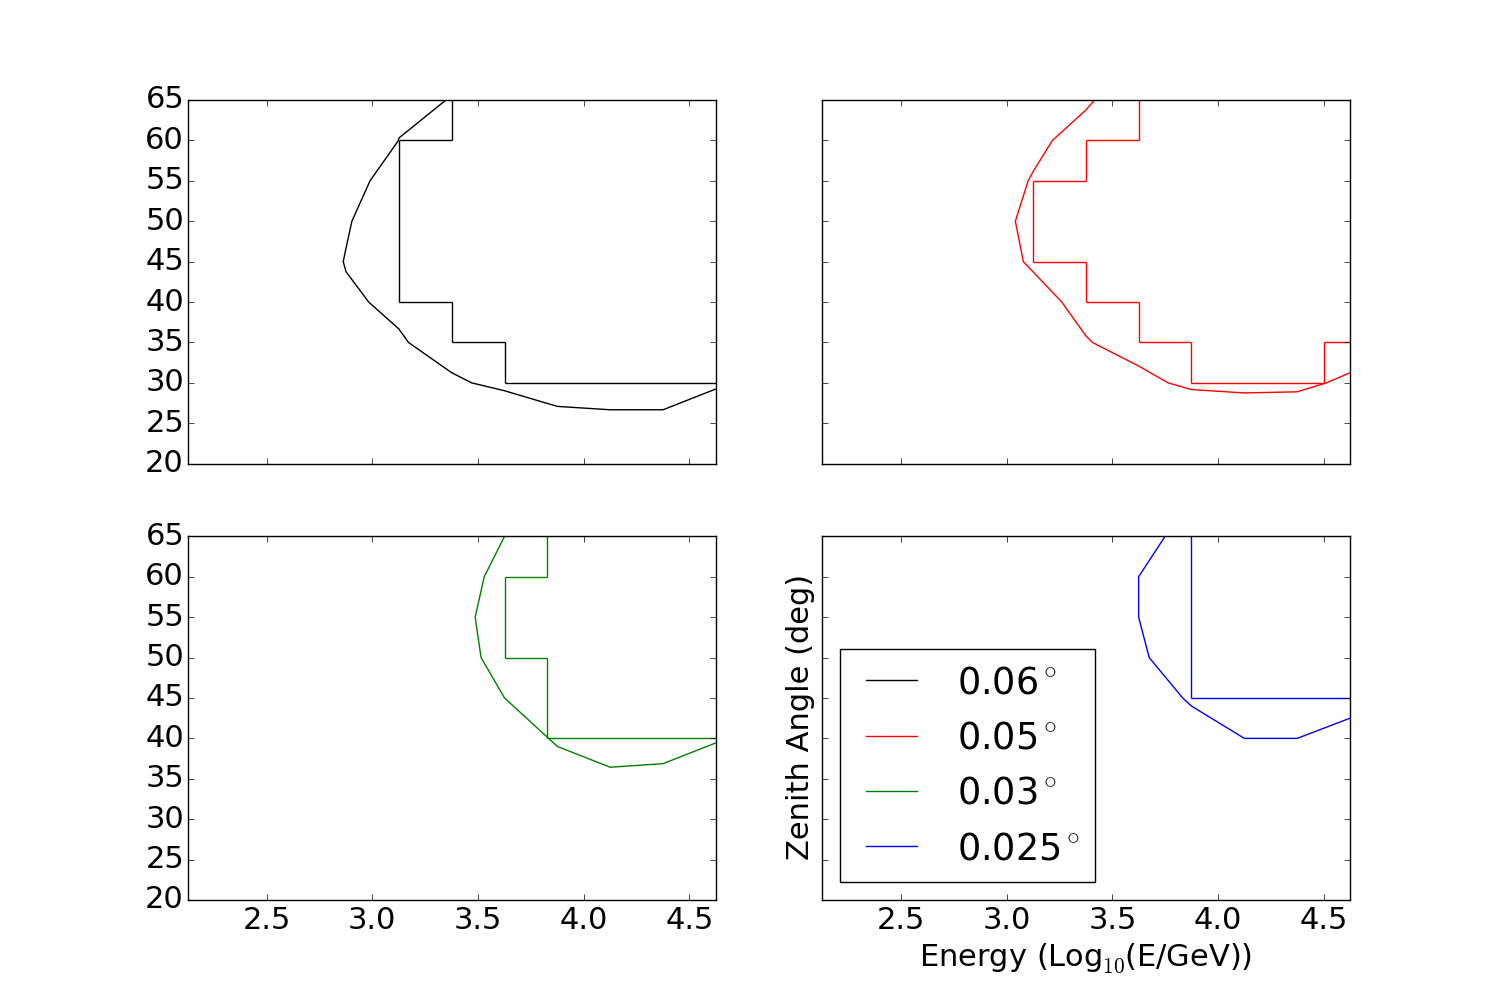
\includegraphics[width=.8\linewidth]{images/boxplot}
%   \caption[Energy and zenith contours for the new Method5t.]{Contours for parameter space with the underestimating-box-sum of conditions used to select relevant events for a comparison with data. The contours correspond to $0.06^\circ$ (upper-left), $0.05^\circ$ (upper-right), $0.03^\circ$ (bottom-left) and $0.025^\circ$ (bottom-right).}
%   \label{fig:contour_boxplot}
% \end{figure}

\section{\rse for the Crab}

The Crab is expected to have a GeV-TeV extension of $\sim 0.03^\circ$ \cite{Fermi_LAT_Crab_extension}\cite{HESS_Crab_extension}. For this, a \rse of at least $0.03^\circ$ is required. This is achieved at zenith angles of $45^\circ$ and greater and above $10^{4}$ GeV. Due to small number statistics in this region of parameter space, the criteria for this work were loosened to include zenith above $40^\circ$ and energies above $10^{3.5}$ GeV. Although this \rse is expected to be insufficient to \textit{measure} the GeV-TeV extension of the Crab due to low statistics, this can be used to demonstrate it \cite{Yeung:energy_extension}.

% \begin{table}[htbp]
%   \begin{center}
%     \begin{tabularx}{\textwidth}{ X | X | X | X | X }
%       \hline
%       \textbf{Min. Zenith (deg)} & \textbf{Min. Energy (TeV)} & \textbf{Min. Energy (Log$_{10}$($\frac{E}{GeV}$))} & \textbf{\rse (deg)} & \textbf{N$_{\rm{on}}$}\\
%       \hline\hline
%       45 & 10.0 & 4.0 & $0.055 \pm 0.008$ & 155\\
%       40 & 3.16 & 3.5 & $0.048 \pm 0.001$ & 913\\
%       40 & 1.0 & 3.0 & $0.1 \pm 4.0$ & 3364\\
%     \end{tabularx}
%     \caption[\rse for the Crab.]{\rse for the Crab from a live time of 35 hours.}
%     \label{tab:crab_res}
%   \end{center}
% \end{table}

\begin{table}[htbp]
  \begin{center}
    \begin{tabularx}{\textwidth}{ X | X | X | X }
      \hline
      \textbf{Contour \#} & \textbf{Simulated \rse (deg)} & \textbf{\rse (deg)} & \textbf{N$_{\rm{on}}$}\\
      \hline\hline
      1 & $0.025$ & $0.046 \pm 0.0008$ & 796\\
       2 & $0.03$ & $0.047 \pm 0.0006$ & 1577\\
      3 & $0.05$ & $0.047 \pm 0.0003$ & 5251\\
      4 & $0.06$ & $0.048 \pm 0.0003$ & 6262\\
    \end{tabularx}
    \caption[\rse for the Crab.]{\rse for the Crab from a live time of 35 hours.}
    \label{tab:crab_res_contour}
  \end{center}
\end{table}

The numbers for the Crab in Table \ref{tab:crab_res} suggest that, if the \rse calculated for simulations is valid for data, we can detect the extension of the Crab. In order to test this, a known point-source with sufficient data collection at LZA and a hard spectrum (and therefore high statistics in the TeV range) was needed. Objects considered for this were Mrk421 and PKS1510-089.

\section{\rse for Mrk421}
Mrk421 is an extra-galactic source ($z=0.031$) with a hard spectrum (spectral index $\Gamma=2.2$), but less than 5 hours of observation in the zenith range of interest ($\phi>40$). 

% \begin{table}[htbp]
%   \begin{center}
%     \begin{tabularx}{\textwidth}{ X | X | X | X | X }
%       \hline
%       \textbf{Min. Zenith (deg)} & \textbf{Min. Energy (TeV)} & \textbf{Min. Energy (Log$_{10}$($\frac{E}{GeV}$))} & \textbf{\rse (deg)} & \textbf{N$_{\rm{on}}$}\\
%       \hline\hline
%       45 & 10.0 & 4.0 & $0.8 \pm 2.0$ & 11\\
%       40 & 3.16 & 3.5 & $0.06 \pm 4.2$ & 328\\
%       40 & 1.0 & 3.0 & $0.047 \pm 0.0006$ & 1850\\
%     \end{tabularx}
%     \caption[\rse for Mrk421.]{\rse for Mrk421 from a live time of 4.62 hours.}
%   \end{center}
% \end{table}

\begin{table}[htbp]
  \begin{center}
    \begin{tabularx}{\textwidth}{ X | X | X | X }
      \hline
      \textbf{Contour \#} & \textbf{Simulated \rse (deg)} & \textbf{\rse (deg)} & \textbf{N$_{\rm{on}}$}\\
      \hline\hline
      1 & $0.025$ & $0.044 \pm 0.002$ & 174\\
      2 & $0.03$ & $0.045 \pm 0.001$ & 489\\
      3 & $0.05$ & $0.051 \pm 0.0005$ & 2914\\
      4 & $0.06$ & $0.050 \pm 0.0004$ & 4556\\
      5 & $0.075$ & $0.048 \pm 0.0003$ & 5989\\
      6 & $0.1$ & $0.048 \pm 0.0002$ & 9984\\
      7 & $0.2$ & $0.048 \pm 0.0002$ & 19005\\
      8 & $0.3$ & $0.048 \pm 0.0002$ & 22127\\
    \end{tabularx}
    \caption[\rse for Mrk 421.]{\rse for Mrk421 from a live time of 35 hours.}
    \label{tab:mrk421_res_contour}
  \end{center}
\end{table}

\section{\rse for PKS1510-089}
PKS1510-089 is an extra-galactic source ($z=0.361$) with a softer spectrum (spectral index $\Gamma=3.26$), but 17 hours of observation in the zenith range of interest ($\phi>40$). Analysis of the data reveals that none of this falls in the region of best performance ($\phi>45$ and $E>10$TeV)

\begin{table}[htbp]
  \begin{center}
    \begin{tabularx}{\textwidth}{ X | X | X | X | X }
      \hline
      \textbf{Min. Zenith (deg)} & \textbf{Min. Energy (TeV)} & \textbf{Min. Energy (Log$_{10}$($\frac{E}{GeV}$))} & \textbf{\rse (deg)} & \textbf{N$_{\rm{on}}$}\\
      \hline\hline
      45 & 10.0 & 4.0 & N/A & 0\\
      40 & 3.16 & 3.5 & $0.7 \pm 2.0$ & 24\\
      40 & 1.0 & 3.0 & $0.09 \pm 0.02$ & 128\\
    \end{tabularx}
    \caption[\rse for PKS1510-089.]{\rse for PKS1510-089 from a live time of 17.1 hours.}
  \end{center}
\end{table}

\end{document}
